\باب{تابع وقت نظریہ اضطراب}\شناخت{باب_تابع_وقت_نظریہ_اضطراب}
%this chapter's typing is complete 

اب تک ہم جو کچھ کر چکے ہیں اس کو \اصطلاح{کوانٹائی سکونیات}\فرہنگ{کوانٹائی سکونیات}\حاشیہب{quantum statics}\فرہنگ{quantum statics} کہا جا سکتا ہے، جس میں مخفی توانائی تفاعل غیر تابع وقت: \عددی{V(\kvec{r}, t)=V(\kvec{r})} ہے۔ ایسی صورت میں ( تابع وقت) مساوات شروڈنگر:
\begin{align*}
	H\Psi=i\hslash\frac{\partial\psi}{\partial t}
\end{align*}
کو علیحدگی متغیرات:
\begin{align*}
	\Psi(\kvec{r}, t) = \psi(\kvec{r})e^{-iEt/\hslash}
\end{align*}
 سے حل کیا جا سکتا ہے، جہاں \عددی{\psi(\kvec{r})} غیر تابع مساوات شروڈنگر	
\begin{align*}
	H\psi=E\psi
\end{align*}
کو مطمئن کرتا ہے۔ چونکہ علیحدگی حلوں میں تابعیت وقت کو قوت نمائی جزو ضربی \عددی{(e^{iEt/\hslash})} ظاہر کرتا ہے، جو کسی بھی طبیعی مقدار \عددی{\abs{\Psi}^2} کے حصول میں منسوخ ہوتا ہے، لہٰذا تمام احتمالات اور توقعاتی قیمتیں وقت کے لحاظ سے مستقل ہوں گے۔ ان ساکن حالات کے \ترچھا{ خطی جوڑ} سے ہم زیادہ دلچسپ تابعیت وقت والے تفاعلات موج تیار کر سکتے ہیں، لیکن اب بھی توانائی اور ان کے متعلقہ احتمالات مستقل ہوں گے۔

توانائی کی ایک سطح سے دوسری سطح میں الیکٹران کی \اصطلاح{ تحویلات} ( جنہیں بعض اوقات \اصطلاح{کوانٹائی چھلانگ}\فرہنگ{کوانٹائی چھلانگ}\حاشیہب{quantum jumps}\فرہنگ{quantum jumps} کہتے ہیں) ممکن بنانے کی خاطر، ضروری ہے کہ ہم \ترچھا{ تابع وقت} مخفیہ (\اصطلاح{کوانٹائی حرکیات}\فرہنگ{کوانٹائی حرکیات}\حاشیہب{quantum dynamics}\فرہنگ{quantum dynamics}) متعارف کریں۔ کوانٹائی حرکیات میں ایسے بہت کم مسائل پائے جاتے ہیں جن کا بالکل ٹھیک ٹھیک حل معلوم کیا جا سکتا ہے۔ ہاں، اگر ہیملٹنی کے غیر تابع وقت حصہ کے لحاظ سے تابع وقت حصہ بہت چھوٹا ہو، تب اسے اضطراب تصور کیا جا سکتا ہے۔ اس باب میں، میں تابع وقت نظریہ اضطراب تیار کرتا ہوں، اور اس کی دو اہم ترین استعمال: جوہر سے اشعاعی اخراج اور انجذاب، پر غور کرتا ہوں۔

\حصہ{دو سطحی نظام}
شروعات کرنے کی غرض سے فرض کریں (غیر مضطرب) نظام کے صرف دو حالات \عددی{\psi_a} اور \عددی{\psi_b} پائے جاتے ہیں۔ یہ غیر مضطرب ہیملٹنی، \عددی{H^0}، کے امتیازی حالات:
\begin{align}\label{مساوات_تابع_مضطرب_دو_سطحی}
	H^0\psi_b=E_b\psi_b ,&&\text{\RL{اور}}&&H^0\psi_a=E_a\psi_a
\end{align}
ہوں گے جو معیاری عمودی ہیں۔
\begin{align}\label{مساوات_تابع_مضطرب_عمودیت}
	\langle\psi_a|\psi_b\rangle=\delta_{ab}
\end{align}
کسی بھی حال کو ان کا خطی جوڑ لکھا جا سکتا ہے؛ بالخصوص، درج ذیل ہو گا۔
\begin{align}
	\Psi(0)=c_a\psi_a+c_b\psi_b
\end{align}

اس سے فرق نہیں پڑتا کہ تفاعلات \عددی{\psi_a} اور \عددی{\psi_b} مقام و فضائی تفاعلات، یا چکر کار، یا کوئی اور عجیب تفاعل ہوں؛ ہمیں یہاں صرف تابعیت \ترچھا{وقت} سے غرض ہے، لہٰذا جب میں \عددی{\Psi(t)} لکھتا ہوں، میرا مراد وقت \عددی{t} پر نظام کا حال ہے۔ عدم اضطراب کی صورت میں، ہر جزو اپنی خصوصی قوت نمائی جزو ضربی کے ساتھ ارتقا:
\begin{align}
	\Psi(t)=c_a\psi_ae^{-iE_at/\hslash}+c_b\psi_be^{-iE_bt/\hslash}
\end{align}
پائے گا۔ ہم کہتے ہیں کہ \قول{حال \عددی{\psi_a} میں ذرہ پائے جانے کا احتمال} \عددی{\abs{c_a}^2} ہے؛ جس سے ہمارا مطلب دراصل یہ ہے کہ پیمائش سے توانائی کی قیمت \عددی{E_a} حاصل ہونے کا احتمال \عددی{\abs{c_a}^2} ہے۔یقیناً، تفاعل \عددی{\Psi} کی معمول زنی کے تحت درج ذیل ہوگا۔
\begin{align}\label{مساوات_تابع_مضطرب_معمول_زنی}
	\abs{c_a}^2+\abs{c_b}^2=1
\end{align}
\جزوحصہ{مضطرب نظام}
 فرض کریں، اب ہم تابع وقت اضطراب، \عددی{H'(t)}، چالو کرتے ہیں۔ چونکہ \عددی{\psi_a} اور \عددی{\psi_b} ایک مکمل سلسلہ قائم کرتے ہیں، لہٰذا تفاعل موج \عددی{\Psi(t)} کو بھی ان کا خطی جوڑ لکھا جا سکتا ہے۔ فرق صرف اتنا ہو گا کہ اب \عددی{c_a} اور \عددی{c_b} وقت \عددی{t} کے \ترچھا{تفاعلات} ہوں گے۔
\begin{align}\label{مساوات_تابع_مضطرب_وقت}
	\Psi(t)=c_a(t)\psi_ae^{-iE_at/\hslash}+c_b(t)\psi_be^{-E_bt/\hslash}
\end{align}
(میں قوت نمائی جزو ضربیوں کو \عددی{c_a(t)} یا \عددی{c_b(t)} میں ضم کر سکتا ہوں، جیسا بعض لوگ کرنا پسند کرتے ہیں، لیکن میں چاہتا ہوں کے تابعیت وقت کا وہ حصہ جو \ترچھا{عدم} اضطراب کی صورت میں بھی پایا جاتا ہو نظر آتا رہے۔) ہمارا پورا کام صرف اتنا ہے کہ ہم وقت کے تفاعلات \عددی{c_a} اور \عددی{c_b} کا تعین کریں۔ مثال کے طور پر، اگر ایک ذرہ آغاز میں حال \عددی{\psi_a} 
(\عددیء{c_a(0)=1}، \عددی{c_b(0)=0}) میں پایا جاتا ہو اور بعد میں کسی وقت \عددی{t_1} پر \عددیء{c_a(t_1)=0}، \عددی{c_b(t_1)=1} ہوں، تب ہم کہیں گے کہ نظام \عددی{\psi_a} سے \عددی{\psi_b} میں تحویل ہوا ہے۔

ہم \عددی{c_a(t)} اور \عددی{c_b(t)} معلوم کرنے کی غرض سے مطالبہ کرتے ہیں کہ \عددی{\Psi(t)} تابع وقت مساوات شروڈنگر کو مطمئن کرے۔
\begin{align}\label{مساوات_تابع_مضطرب_مطمئن}
	H\Psi=i\hslash\frac{\partial\Psi}{\partial t},&&H=H^0+H'(t)
\end{align}
مساوات \حوالہ{مساوات_تابع_مضطرب_وقت} اور مساوات \حوالہ{مساوات_تابع_مضطرب_مطمئن} سے درج ذیل حاصل ہوگا۔
\begin{multline*}
	c_a[H^0\psi_a]e^{-iE_at/\hslash}+c_b[H^0\psi_b]e^{-iE_bt/\hslash}+c_a[H'\psi_a]e^{-iE_at/\hslash}+c_b[H'\psi_b]e^{-iE_bt/\hslash} \\
	=i\hslash\Big[\dot{c}_a\psi_ae^{-iE_at/\hslash}+\dot{c}_b\psi_be^{-iE_bt/\hslash}\\
	+c_a\psi_a\left(-\frac{iE_a}{\hslash}\right)e^{-iE_at/\hslash}+c_b\psi_b\left(-\frac{iE_b}{\hslash}\right)e^{-iE_bt/\hslash}\Big]
\end{multline*}
مساوات \حوالہ{مساوات_تابع_مضطرب_دو_سطحی} کی بدولت بائیں ہاتھ کے پہلے دو اجزاء دائیں ہاتھ کے آخری دو اجزاء کے ساتھ کٹتے ہیں، لہٰذا درج ذیل رہ جائے گا۔
\begin{align}
	c_a[H'\psi_a]e^{-iE_at/\hslash}+c_b[H'\psi_b]e^{-iE_bt/\hslash}=i\hslash\left[\dot{c}_a\psi_ae^{-iE_at/\hslash}+\dot{c}_b\psi_be^{-iE_bt/\hslash}\right]
\end{align}

تفاعل \عددی{\psi_a} کے ساتھ اندرونی ضرب لے کر \عددی{\psi_a} اور \عددی{\psi_b} کی عمودیت ( مساوات \حوالہ{مساوات_تابع_مضطرب_عمودیت}) بروئے کار لاتے ہوئے ہم \عددی{\dot{c}_a} کو الگ کرتے ہیں۔
\begin{align*}
	c_a\langle\psi_a| H'|\psi_a\rangle e^{-iE_at/\hslash}+c_b\langle\psi_a| H'|\psi_b\rangle e^{-iE_bt/\hslash}=i\hslash\dot{c}_ae^{-iE_at/\hslash}
\end{align*}
مختصر لکھائی کے غرض سے ہم درج ذیل متعارف کرتے ہیں:
\begin{align}
	H'_{ij}\equiv\langle\psi_i| H'|\psi_j\rangle
\end{align}
دھیان رہے کہ \عددی{H'} ہرمشی ہے، لہٰذا \عددی{H'_{ji}=(H'_{ij})^*} ہوگا۔ دونوں اطراف کو \عددی{-(i/\hslash)e^{iE_at/\hslash}} سے ضرب دے کر درج ذیل حاصل ہوگا۔
\begin{align}\label{مساوات_تابع_مضطرب_تحویلی_شرح_الف}
	\dot{c}_a=-\frac{i}{\hslash}\left[c_aH'_{aa}+c_bH'_{ab}e^{-i(E_b-E_a)t/\hslash}\right]
\end{align}
اسی طرح \عددی{\psi_b} کے ساتھ اندرونی ضرب سے \عددی{\dot{c}_b} الگ کیا جا سکتا ہے:
\begin{align*}
	c_a\langle\psi_b| H'|\psi_a\rangle e^{-iE_at/\hslash}+c_b\langle\psi_b| H'|\psi_b\rangle e^{-iE_bt/\hslash}=i\hslash\dot{c}_be^{-iE_bt/\hslash}
\end{align*}
لہٰذا درج ذیل ہوگا۔
\begin{align}\label{مساوات_تابع_مضطرب_تحویلی_شرح_ب}
	\dot{c}_b=-\frac{i}{\hslash}\left[c_bH'_{bb}+c_aH'_{ba}e^{i(E_b-E_a)t/\hslash}\right]
\end{align}

مساوات \حوالہ{مساوات_تابع_مضطرب_تحویلی_شرح_الف} اور مساوات \حوالہ{مساوات_تابع_مضطرب_تحویلی_شرح_ب} مل کر \عددی{c_a(t)} اور \عددی{c_b(t)} کا تعین کرتے ہیں؛ یہ دونوں مل کر دو سطحی نظام کی (تابع وقت) مساوات شروڈنگر کے مکمل معادل ہیں۔ عمومی طور پر \عددی{H'} کے وتری قالبی ارکان صفر ہوں گے:
\begin{align}
	H'_{aa}=H'_{bb}=0
\end{align}
 (عمومی صورت کے لیے سوال \حوالہ{سوال_تابع_مضطرب_عمومی_صورت} دیکھیں)۔ اگر ایسا ہو تب مساوات سادہ روپ:
\begin{align}\label{مساوات_تابع_مضطرب_شرح_ضربیات}
	\dot{c}_a=-\frac{i}{\hslash}H'_{ab}e^{-i\omega_0t}c_b,&&\dot{c}_b=-\frac{i}{\hslash}H'_{ba}e^{i\omega_0t}c_a
\end{align}
 اختیار کرتی ہے، جہاں درج ذیل ہوگا۔
\begin{align}
	\omega_0\equiv\frac{E_b-E_a}{\hslash}
\end{align}
(میں \عددی{E_b\geq E_a} فرض کرتا ہوں، لہٰذا \عددی{\omega_0\geq0} ہوگا۔)



\ابتدا{سوال}\شناخت{سوال_تابع_مضطرب_تکمل_صفر}
ایک ہائیڈروجن جوہر کو (تابع وقت) برقی میدان \عددی{\kvec{E}=E(t)\ak} میں رکھا جاتا ہے۔ زمینی حال \عددی{(n=1)} اور ( چار گنا انحطاطی) پہلے ہیجان حالات \عددی{(n=2)} کے بیچ اضطراب \عددی{H'=eEz} کے چاروں قالبی ارکان \عددی{H'_{ij}} تلاش کریں۔ دکھائیں کہ پانچوں حالات کے لیے \عددی{H'_{ii}=0} ہوگا۔ \ترچھا{تبصرہ:} محور \عددی{z} کے لحاظ سے \اصطلاح{طاق پن}\فرہنگ{طاق پن}\حاشیہب{oddness}\فرہنگ{oddness} کو بروئے کار لاتے ہوئے، صرف ایک تکمل حل کرنے کی ضرورت ہو گی؛ اس روپ کا اضطراب زمینی حال سے \عددی{n=2} حالات میں سے صرف ایک تک رسائی دیتا ہے، لہٰذا یہ نظام دو حالات تشکیل کے طور پر کام کرے گا؛ یہاں فرض کیا گیا ہے کہ بلند ہیجان حالات تک تحویل نظر انداز کی جا سکتی ہے۔
\انتہا{سوال}
\ابتدا{سوال}\شناخت{سوال_تابع_مضطرب_غیر_تابع}
\ترچھا{غیر تابع وقت} اضطراب کی صورت میں \عددی{c_a(0)=1} اور \عددی{c_b(0)=0} لیتے ہوئے مساوات \حوالہ{مساوات_تابع_مضطرب_شرح_ضربیات} حل کریں۔ تصدیق کریں کہ \عددی{\abs{c_a(t)}^2+\abs{c_b(t)}^2=1} ہے۔ \ترچھا{ تبصرہ:} بظاہر یہ نظام \قول{خالص \عددی{\psi_a}} اور \قول{کسی \عددی{\psi_b}} کے بیچ ارتعاش کرتا ہے۔ کیا یہ میرے اس عمومی دعوے کی نفی نہیں کرتا کہ غیر تابع وقت اضطراب کی صورت میں تحویل نہیں ہوگی؟ جی نہیں، لیکن اس کی وجہ کچھ لطیف ہے: یہاں \عددی{\psi_a} اور \عددی{\psi_b} نہ کبھی ہیملٹنی کے امتیازی تفاعلات تھے اور نہ ہیں؛ توانائی کی پیمائش کبھی بھی \عددی{E_a} یا \عددی{E_b} نہیں دیگی۔نظام پر نظر ڈالنے کی خاطر، تابع وقت نظریہ اضطراب میں ہم عموماً اضطراب \ترچھا{ چالو} کر کے کچھ دورانیہ کے بعد \ترچھا{بند} کرتے ہیں۔ آغاز اور اختتام میں \عددی{\psi_a} اور \عددی{\psi_b} بالکل ٹھیک ہیملٹنی کے امتیازی حالات ہوں گے، اور صرف اس سیاق و سباق میں ہم کہہ سکتے ہیں کہ نظام ایک سے دوسرے میں تحویل ہوا۔ یوں، موجودہ مسئلے میں، فرض کریں کہ وقت \عددی{t=0} پر اضطراب چالو کیا جاتا ہے جسے وقت \عددی{t} پر بند کیا جاتا ہے؛ اس سے حساب پر کوئی فرق نہیں پڑے گا، تاہم یہ نتائج کی معقول تشریح ممکن بناتی ہے۔
\انتہا{سوال}
\ابتدا{سوال}
فرض کریں اضطراب کا روپ (وقت کا) \عددی{\delta} تفاعل ہے۔
\begin{align*}
	H'=U\delta(t) 
\end{align*}
فرض کریں \عددی{U_{aa}=U_{bb}=0} اور \عددی{U_{ab}=U^*_{ba}\equiv\alpha} ہے۔ اگر \عددی{c_a(-\infty)=1} اور \عددی{c_b(-\infty)=0} ہوں، \عددی{c_a(t)} اور \عددی{c_b(t)} تلاش کریں، اور تصدیق کریں کہ \عددی{\abs{c_a(t)}^2+\abs{c_b(t)}^2=1} ہے۔ تحویل ہونے کا خالص احتمال ( \عددی{t\to\infty} کے لیے \عددی{P_{a\to b}}) کیا ہوگا؟ \ترچھا{ اشارہ:} آپ ڈیلٹا تفاعل کو مستطیلوں کے تسلسل کی تحدیدی حد لے سکتے ہیں۔

جواب: \عددی{P_{a\to b}=\sin^2(|\alpha|/\hslash)} 
\انتہا{سوال}


\جزوحصہ{تابع وقت نظریہ اضطراب}
اب تک سب کچھ بالکل ٹھیک رہا ہے: ہم نے اضطراب کی جسامت کے بارے میں کچھ فرض نہیں کیا۔ لیکن، \قول{چھوٹے} \عددی{H'} کی صورت میں ہم مساوات \حوالہ{مساوات_تابع_مضطرب_شرح_ضربیات} کو (درج ذیل) یک بعد دیگر تخمین سے حل کر سکتے ہیں۔ فرض کریں ذرہ زیریں حال:
\begin{align}
	c_a(0)=1,\quad c_b(0)=0
\end{align}
سے آغاز کرتا ہے۔ عدم اضطراب کی صورت میں ذرہ ہمیشہ کے لیے یہیں ( صفر رتبی میں) رہے گا۔

\موٹا{ صفر رتبی:}
\begin{align}
	c^{(0)}_a(t)=1,\quad c_b^{(0)}(t)=0
\end{align}
(میں تخمین کے رتبہ کو زیر بالا میں قوسین میں لکھتا ہوں۔ یوں \عددی{c_a^{(0)}(t)} میں \عددی{\قول{0}} رتبہ صفر کو ظاہر کرتا ہے۔)

ہم مساوات \حوالہ{مساوات_تابع_مضطرب_شرح_ضربیات} کے دائیں ہاتھ میں رتبہ صفر قیمتیں پُر کر کے اول رتبی تخمین حاصل کرتے ہیں۔

\موٹا{ اول رتبی:}
\begin{gather}
\begin{aligned}\label{مساوات_تابع_مضطرب_اول_رتبی}
		\frac{\dif c_a^{(1)}}{\dif t}=0&\to c_a^{(1)}(t)=1 \\
		\frac{\dif c_b^{(1)}}{\dif t}=-\frac{i}{\hslash}H'_{ba}e^{i\omega_0t}&\to c_b^{(1)}=-\frac{i}{\hslash}\int_{0}^{t}H'_{ba}(t')e^{i\omega_0t'}\dif t'
\end{aligned}
\end{gather}
اب ہم انہیں دائیں ہاتھ میں پُر کر کے رتبہ دوم تخمین حاصل کرتے ہیں۔

\موٹا{دوم رتبی:}	
\begin{multline}
		\frac{\dif c_a^{(2)}}{\dif t}=-\frac{i}{\hslash}H'_{ab}e^{-i\omega_0t}\left(-\frac{i}{\hslash}\right)\int_{0}^{t}H'_{ba}(t')e^{i\omega_0t'}\dif t'\to \\
		c_a^{(2)}(t)=1-\frac{1}{\hslash^2}\int_{0}^{t}H'_{ab}(t')e^{-i\omega_0t'}\left[\int_{0}^{t'}H'_{ba}(t'')e^{i\omega_0t''}\dif t''\right]\dif t'
\end{multline}
جہاں \عددی{c_b} تبدیل نہیں ہوا \عددی{(c^{(2)}_b(t)=c^{(1)}_b(t))}۔ ( دھیان رہے کہ \عددی{c^{(2)}_a(t)} میں صفر رتبی جزو بھی شامل ہے؛ دوم رتبی \ترچھا{تصحیح} صرف تکملی حصہ ہوگا۔)

اصولاً، ہم اسی طرح چلتے ہوئے \عددی{n} رتبی تخمین کو مساوات \حوالہ{مساوات_تابع_مضطرب_شرح_ضربیات} کے دائیں ہاتھ میں پُر کر کے \عددی{(n+1)} رتبی تخمین کے لیے حل کر سکتے ہیں۔صفر رتبی میں \عددی{H'} کا کوئی جزو ضربی نہیں پایا جاتا، اول رتبی تصحیح میں \عددی{H'} کا ایک جزو ضربی پایا جاتا ہے، دوم رتبی تصحیح میں \عددی{H'} کے دو جزو ضربی پائے جاتے ہیں، وغیرہ۔\حاشیہد{دھیان رہے کہ ہر جفت رتبہ میں \عددی{c_a}، اور ہر طاق رتبہ میں \عددی{c_b}تبدیل ہوتا ہے؛ اگر نظام ان دو حالات کے خطی جوڑ سے آغاز کرے، یا اضطراب میں وتری ارکان پائے جائیں، تب ایسا نہیں ہو گا۔} اول رتبی تخمین میں سہو 
 \عددی{|c^{(1)}_a(t)|^2+|c^{(1)}_b(t)|^2\neq1} سے صاف ظاہر ہے ( ٹھیک عددی سروں کو یقیناً مساوات \حوالہ{مساوات_تابع_مضطرب_معمول_زنی} پر پورا اترنا ہوگا)۔ ہاں \عددی{H'} میں اول رتبہ تک \عددی {|c^{(1)}_a(t)|^2+|c^{(1)}_b(t)|^2} کی قیمت \عددی{1} ہو گی؛ اول رتبی تخمین سے اتنی ہی توقع کی جا سکتی ہے۔ یہی کچھ زیادہ بلند رتبی تخمین کے لیے بھی ہوگا۔

\ابتدا{سوال}\شناخت{سوال_تابع_مضطرب_عمومی_صورت}
فرض کریں آپ \عددی{H'_{aa}=H'_{bb}=0} نہیں لیتے۔
\begin{enumerate}[a.]
\item
 صورت \عددی{c_a(0)=1} اور \عددی{c_b(0)=0} کے لئے اول رتبی نظریہ اضطراب سے \عددی{c_a(t)} اور \عددی{c_b(t)} حاصل کریں۔ دکھائیں کہ \عددی{H'} میں اول رتبہ تک
 \عددی {|c^{(1)}_a(t)|^2+|c^{(1)}_b(t)|^2=1} ہو گا۔
\item
 اس مسئلے کو بہتر انداز میں نمٹا جا سکتا ہے۔ درج ذیل لیکر
\begin{align}
	d_a\equiv e^{\frac{i}{\hslash}\int_{0}^{t}H'_{aa}(t')\dif t'}c_a,&&d_b\equiv e^{\frac{i}{\hslash}\int_{0}^{t}H'_{bb}(t')\dif t'}c_b
\end{align}
دکھائیں کہ
\begin{align}
	\dot{d}_a=-\frac{i}{\hslash}e^{i\phi}H'_{ab}e^{-i\omega_0t}d_b;&&\dot{d}_b=-\frac{i}{\hslash}e^{-i\phi}H'_{ba}e^{i\omega_0t}d_a
\end{align}
ہو گا، جہاں درج ذیل ہے۔
\begin{align}
	\phi(t)\equiv\frac{1}{\hslash}\int_{0}^{t}[H'_{aa}(t')-H'_{bb}(t')]\dif t'
\end{align}
یوں ( \عددی{H'} کے ساتھ چسپاں اضافی جزو ضرب \عددی{e^{i\phi}} کے علاوہ) \عددی{d_a} اور \عددی{d_b} کی مساواتیں، ساخت کے لحاظ سے مساوات \حوالہ{مساوات_تابع_مضطرب_شرح_ضربیات} کی متماثل ہیں۔
\item
 اول رتبی نظریہ اضطراب سے، جزو -ب کی ترکیب استعمال کرتے ہوئے، \عددی{c_a(t)} اور \عددی{c_b(t)} حاصل کریں، اور اپنے جواب کا جزو-الف کے ساتھ موازنہ کریں۔ دونوں میں فرق پر تبصرہ کریں۔
 \end{enumerate}
\انتہا{سوال}
\ابتدا{سوال}
عمومی صورت \عددی{c_a(0)=a}، \عددی{c_b(0)=b} کے لیے نظریہ اضطراب میں مساوات \حوالہ{مساوات_تابع_مضطرب_شرح_ضربیات} کو دوم رتبہ تک حل کریں۔
\انتہا{سوال}
\ابتدا{سوال}
غیر تابع وقت اضطراب (سوال \حوالہ{سوال_تابع_مضطرب_غیر_تابع}) کے لیے \عددی{c_a(t)} اور \عددی{c_b(t)} کو دوم رتبہ تک حاصل کریں۔ اپنے جواب کا ٹھیک ٹھیک نتیجے کے ساتھ موازنہ کریں۔
\انتہا{سوال}
%==================

\جزوحصہ{سائن نما اضطراب}\شناخت{حصہ_تابع_مضطرب_سائن_نما_اضطراب}
فرض کریں اضطراب میں تابعیت وقت سائن نما ہو: 
\begin{align}
	H'(\kvec{r}, t) = V(\kvec{r})\cos(\omega t)
\end{align}
تب 
\begin{align}
	H'_{ab}=V_{ab}\cos(\omega t)
\end{align}
ہو گا، جہاں \عددی{V_{ab}} درج ذیل ہے۔
\begin{align}
	V_{ab}\equiv\langle\psi_a| V|\psi_b\rangle
\end{align}
(عملاً، تقریباً ہر صورت میں وتری قالبی ارکان صفر ہوتے ہیں، لہٰذا پہلے کی طرح یہاں بھی میں فرض کرتا ہوں کہ وتری قالبی ارکان صفر ہیں۔) اول رتبہ تک (یہاں سے آگے، ہم صرف اول رتبہ تک کام کریں گے، لہٰذا زیر بالا میں رتبہ کی نشاندہی نہیں کی جائے گی)) درج ذیل ہوگا (مساوات \حوالہ{مساوات_تابع_مضطرب_اول_رتبی})۔
\begin{align}\label{مساوات_تابع_مضطرب_دو_اجزاء}
	c_b(t) &\cong-\frac{i}{\hslash}V_{ba}\int_{0}^{t}\cos(\omega t')e^{i\omega_0 t'}\dif t' = -\frac{iV_{ba}}{2\hslash}\int_{0}^{t}\left[e^{i(\omega_0+\omega)t'}+e^{i(\omega_0-\omega)t'}\right]\dif t' \nonumber \\
	&=-\frac{V_{ba}}{2\hslash}\left[\frac{e^{i(\omega_0+\omega)t}-1}{\omega_0+\omega}+\frac{e^{i(\omega_0-\omega)t}-1}{\omega_0-\omega}\right]
\end{align}

یہی جواب ہے، لیکن اس کے ساتھ کام کرنا ذرا دشوار ہوگا۔ جبری تعدد \عددی{(\omega)} کو تحویلی تعدد \عددی{(\omega_0)} کے بہت قریب رہنے کا پابند بنانے سے، چوکور قوسین میں دوسرا جزو غالب ہوگا، جس سے چیزیں نہایت آسان ہو جاتی ہیں؛ بالخصوص ہم درج ذیل فرض کرتے ہیں۔
\begin{align}
	\omega_0+\omega\gg\abs{\omega_0-\omega}
\end{align}
یہ بہت بڑی پابندی نہیں ہے، چونکہ کسی دوسرے تعدد پر تحویل کا احتمال نہ ہونے کے برابر ہے۔\حاشیہد{آنے والے حصوں میں ہم اس نظریے کا اطلاق روشنی پر کریں گے، جس 
کا \عددی{\omega\sim \SI{e15}{\per\second}} ہے، لہٰذا دونوں اجزاء میں نسب نما انتہائی بڑا ہو گا، ماسوائے \عددی{\omega_0} کے قریب (دوسرے جزو میں)۔} پہلے جزو کو نظرانداز کرتے ہوئے درج ذیل لکھا جا سکتا ہے۔
\begin{align}
	c_b(t) &\cong-\frac{V_{ba}}{2\hslash}\frac{e^{i(\omega_0-\omega)t/2}}{\omega_0-\omega}\left[e^{i(\omega_0-\omega)t/2}-e^{-i(\omega_0-\omega)t/2}\right]\nonumber \\
	&=-i\frac{V_{ba}}{\hslash}\frac{\sin[(\omega_0-\omega)t/2]}{\omega_0-\omega}e^{i(\omega_0-\omega)t/2}
\end{align}
ایک ذرہ جو حال \عددی{\psi_a} سے آغاز کر کے لمحہ\عددی{t} پر حال \عددی{\psi_b} میں پایا جاتا ہو، کے تحویل کا احتمال، جس کو \اصطلاح{تحویلی احتمال}\فرہنگ{تحویلی احتمال}\حاشیہب{transition probability}\فرہنگ{transition probability} کہتے ہیں، درج ذیل ہو گا۔
\begin{align}\label{مساوات_تابع_مضطرب_تحویلی_احتمال}
	P_{a\to b}(t)=\abs{c_b(t)}^2\cong\frac{\abs{V_{ab}^2}}{\hslash^2}\frac{\sin^2[(\omega_0-\omega)t/2]}{(\omega_0-\omega)^2}
\end{align}

اس نتیجے کا دلچسپ پہلو یہ ہے کہ، وقت کے لحاظ سے تحویلی احتمال سائن نما \ترچھا{ارتعاش} کرتا ہے (شکل \حوالہ{شکل_تابع_وقت_احتمال_سائن_نما_احتمال})۔
 یہ \عددی{\abs{V_{ab}}^2/\hslash^2(\omega_0-\omega)^2} کی اعظم قیمت تک پہنچ کر، جو لازماً \عددی{1} سے بہت کم ہے ( ورنہ ہم اضطراب کو چھوٹا فرض نہیں کر پائیں گے) یہ واپس گر کر صفر ہوتا ہے! لمحات \عددی{t_n=2n\pi/\abs{\omega_0-\omega}} پر، جہاں \عددی{n=1, 2, 3, \dotsc} ہے، ذرہ لازماً نچلے حال میں ہوگا۔ اگر آپ تحویل کا احتمال بڑھانا چاہتے ہیں، اضطراب کو لمبے عرصے کے لیے چالو نہ رکھیں؛ بہتر ہوگا کہ آپ وقت \عددی{\pi/\abs{\omega_0-\omega}} پر اضطراب کو بند کر کے نظام کو بالائی حال میں \قول{پانے} کی امید کریں۔ سوال \حوالہ{سوال_تابع_مضطرب_بالائی_حال_امید} میں آپ دیکھیں گے کہ دو حالات کے بیچ تحویل، نظریہ اضطراب کی پیدا کردہ مصنوعی خاصیت نہیں، بلکہ ٹھیک حال میں بھی ایسا ہی ہوگا، اگرچہ تحویلی تعدد کچھ مختلف ہوگا۔

\begin{figure}
\centering
\begin{tikzpicture}[declare function={f(\x)= 1-cos(\x);}]
\begin{axis}[axis lines=middle,xlabel={$t$},ylabel={$P(t)$}, xtick={360,720,1080},
 xticklabels={$\tfrac{2\pi}{\abs{\omega_0-\omega}}$ ,$\tfrac{4\pi}{\abs{\omega_0-\omega}}$, $\tfrac{6\pi}{\abs{\omega_0-\omega}}$}, ytick={2}, yticklabels={$\abs{\tfrac{\abs{V_{ab}}}{\hslash(\omega_0-\omega)}}^2$}, ylabel style={at={(current axis.above origin)},anchor=west},xlabel style={at={(current axis.right of origin)},anchor=north east},enlargelimits]
\addplot [thick,samples=100,domain=0:1260]{f(x)};
\addplot [dashed] coordinates{(0,2)(1260,2)};
\end{axis}
\end{tikzpicture}
\caption{سائن نما اضطراب کے لئے وقت کے لحاظ سے تحویلی احتمال (مساوات \حوالہ{مساوات_تابع_مضطرب_تحویلی_احتمال})۔}
\label{شکل_تابع_وقت_احتمال_سائن_نما_احتمال}
\end{figure}


جیسا میں ذکر کر چکا ہوں، تحویل کا احتمال اس صورت سب سے زیادہ ہوگا جب جبری تعدد قدرتی تعدد \عددی{\omega_0} کے قریب ہو۔ شکل \حوالہ{شکل_تابع_وقت_احتمال_جبری_تعدد} میں \عددی{\omega} کے لحاظ سے \عددی{P_{a\to b}} ترسیم کر کے اس حقیقت کو اجاگر کیا گیا ہے۔ چوٹی کی بلندی \عددی{(\abs{V_{ab}}t/2\hslash)^2} جبکہ چوڑائی \عددی{4\pi/t} ہے؛ ظاہر ہے کہ وقت گزرنے کے ساتھ ساتھ اسکی بلندی بڑھتی اور چوڑائی گھٹتی ہے۔ ( بظاہر، اعظم قیمت بغیر کسی حد کی بتدریج بڑھتی ہے۔ تاہم \عددی{1} تک پہنچنے سے بہت پہلے چھوٹے اضطراب کا مفروضہ ناکارہ ہو جاتا ہے، لہٰذا ہم نسبتاً کم \عددی{t} کے لیے اس نتیجے پر یقین کر سکتے ہیں۔ سوال \حوالہ{سوال_تابع_مضطرب_بالائی_حال_امید} میں آپ دیکھیں گے کہ ٹھیک نتیجہ \عددی{1} سے تجاوز نہیں کرتا۔)
\begin{figure}
\centering
\pgfmathsetmacro{\k}{15}
\pgfmathsetmacro{\ka}{\k-2*pi}
\pgfmathsetmacro{\kb}{\k+2*pi}
\begin{tikzpicture}[declare function={f(\x)= (sin(deg(\k-\x)/2)^2)/pow(\k-\x,2);}]
\begin{axis}[clip=false,axis lines=middle,xlabel={$\omega$},ylabel={$P(\omega)$}, xtick={\k,\ka,\kb},
 xticklabels={$\omega_0$,,}, ytick={0.25}, yticklabels={}, ylabel style={at={(current axis.above origin)},anchor= east},xlabel style={at={(current axis.right of origin)},anchor=north},enlargelimits]
\addplot [thick,smooth,domain=0:30,samples=50]{f(x)};
\addplot[] coordinates {(\ka,0)}node[pin=-120:{$(\omega_0-2\pi/t)$}]{};
\addplot[] coordinates {(\kb,0)}node[pin=-60:{$(\omega_0+2\pi/t)$}]{};
\end{axis}
\end{tikzpicture}
\caption{تحویلی احتمال بالمقابل متحرک تعدد (مساوات \حوالہ{مساوات_تابع_مضطرب_تحویلی_احتمال})۔}
\label{شکل_تابع_وقت_احتمال_جبری_تعدد}
\end{figure}


\ابتدا{سوال}\شناخت{سوال_تابع_مضطرب_بالائی_حال_امید}
مساوات \حوالہ{مساوات_تابع_مضطرب_دو_اجزاء} میں پہلا جزو \عددی{\cos(\omega t)} کے \عددی{e^{i\omega t}/2} حصہ سے، اور دوسرا \عددی{e^{-i\omega t}/2} سے آتا ہے۔ یوں پہلے جزو کو نظرانداز کرنا باضابطہ طور پر \عددی{H'=(V/2)e^{-i\omega t}} لکھنے کا معادل ہے، یعنی ہم درج ذیل کہہ سکتے ہیں۔
\begin{align}\label{مساوات_تابع_مضطرب_کوسائن_ایک_جزو}
	H'_{ba}=\frac{V_{ba}}{2}e^{-i\omega t},&&H'_{ab}=\frac{V_{ab}}{2}e^{i\omega t}
\end{align}
(ہیملٹنی قالب کو ہرمشی بنانے کی خاطر موخر الذکر کی ضرورت پیش آتی ہے؛ آپ کہہ سکتے ہیں کہ ہم \عددی{c_a(t)} کے لیے مساوات \حوالہ{مساوات_تابع_مضطرب_دو_اجزاء} کی طرح کلیہ میں غالب جزو منتخب کرتے ہیں۔ ) اس کو \اصطلاح{ گھومتی موج تخمین}\فرہنگ{گھومتی موج تخمین}\حاشیہب{rotating wave approximation}\فرہنگ{rotating wave approximation} کہتے ہیں۔ جناب \موٹا{رابی} نے دیکھا کہ حساب کے آغاز میں گھومتی موج تخمین کرتے ہوئے مساوات \حوالہ{مساوات_تابع_مضطرب_شرح_ضربیات} کو، نظریہ اضطراب استعمال کیے بغیر اور میدان کے زور کے بارے میں کچھ فرض کیے بغیر، بالکل ٹھیک ٹھیک حل کیا جا سکتا ہے۔
\begin{enumerate}[a.]
\item
 عمومی ابتدائی معلومات \عددی{c_a(0)=1}، \عددی{c_b(0)=0} کے لیے گھومتی موج تخمین (مساوات \حوالہ{مساوات_تابع_مضطرب_کوسائن_ایک_جزو}) لیتے ہوئے مساوات \حوالہ{مساوات_تابع_مضطرب_شرح_ضربیات} حل کریں۔ اپنے جوابات ( \عددی{c_a(t)} اور \عددی{c_b(t)}) کو \اصطلاح{ رابی پلٹنی تعدد}:\فرہنگ{رابی پلٹنی تعدد}\حاشیہب{Rabi flopping frequency}\فرہنگ{Rabi flopping frequency} 
\begin{align}
	\omega_r\equiv\frac{1}{2}\sqrt{(\omega-\omega_0)^2+(\abs{V_{ab}}/\hslash)^2}
\end{align}
کی صورت میں لکھیں۔
\item
 تحویلی احتمال \عددی{P_{a\to b}(t)}کا تعین کریں، اور دکھائیں کہ یہ کبھی بھی \عددی{1} سے تجاوز نہیں کرتا۔ تصدیق کریں کہ \عددی {|c_a(t)|^2+|c_b(t)|^2=1} ہے۔
\item
 تصدیق کریں کہ \قول{کم} اضطراب کی صورت میں \عددی{P_{a\to b}(t)} نظریہ اضطراب کا نتیجہ( مساوات \حوالہ{مساوات_تابع_مضطرب_تحویلی_احتمال}) دے گا۔ سیاق و سباق کے لحاظ سے یہاں \قول{کم} سے مراد \عددی{V} پر عائد کیا پابندی ہے۔
\item
 نظام پہلی مرتبہ اپنے ابتدائی حال میں کس وقت واپس آئے گا؟
 \end{enumerate}
\انتہا{سوال}



\حصہ{اشعاعی اخراج اور انجذاب} 
\جزوحصہ{برقناطیسی امواج}
ایک برقناطیسی موج (جس کو میں روشنی کہوں گا، اگرچہ یہ زیریں سرخ، بالائے بصری شعاع، خرد امواج، ایکس رے، وغیرہ ہو سکتی ہے؛ جن میں صرف تعدد کا فرق ہے) عرضی ( اور باہم قائمہ) ارتعاشی برقی اور مقناطیسی میدانوں پر مشتمل ہوگا (شکل \حوالہ{شکل_تابع_وقت_احتمال_برقناطیسی_موج})۔ ایک جوہر، گزرتی ہوئی بصری موج کی برقی جزو کو، بنیادی طور پر ردعمل کرتا ہے۔ اگر طول موج (جوہر کی جسامت کے لحاظ سے) لمبا ہو، ہم میدان کے \اصطلاح{فاصلاتی} تغیر کو نظرانداز کر سکتے ہیں۔\حاشیہد{بصری روشنی کے لئے \عددی{\lambda\sim\SI{500}{\nano\meter}} جبکہ جوہر کا قطر \عددی{\SI{0.1}{\nano\meter}} کے لگ بھگ ہے، لہٰذا یہ تخمین معقول ہے؛ تاہم ایکس رے کے لئے ایسا نہیں ہو گا۔ سوال \حوالہ{سوال_تابع_مضطرب_فاصلاتی_تغیر} میدان کے فاصلاتی تغیر پر غور کرتا ہے۔} تب جوہر سائن نما ارتعاشی برقی میدان:
\begin{align}\label{مساوات_تابع_مضطرب_بہت_چھوٹا_جوہر}
	\kvec{E} = E_0\cos(\omega t)\,\ak
\end{align}
کے زیر اثر ہوگا ( فی الحال میں روشنی کو یک رنگی اور \عددی{z} رخ تقطیب شدہ فرض کرتا ہوں)۔ اضطرابی ہیملٹنی\حاشیہد{ساکن میدان \عددی{\kvec{E}} میں بار \عددی{q} کی توانائی \عددی{-q\int\kvec{E}\cdot\dif\kvec{r}} ہو گی۔ آپ تابع وقت (یعنی غیر ساکن) میدان کے لئے برقی سکونیات کے کلیہ کے استعمال پر ناراض ہو سکتے ہیں۔میں بغیر کہے، فرض کرتا ہوں کہ (جوہر کے اندر) الیکٹران کو حرکت کرنے کے لئے درکار وقت سے ارتعاش کا دوری عرصہ زیادہ ہے۔} درج ذیل ہوگی، جہاں \عددی{q} الیکٹران کا بار ہے۔\حاشیہد{ہمیشہ کی طرح ہم فرض کرتے ہیں کہ مرکزہ بھاری اور ساکن ہے؛ ہمیں یہاں الیکٹران کے تفاعل موج سے غرض ہے۔}
\begin{align}
	H'=-qE_0z\cos(\omega t)
\end{align}	
%
\begin{figure}
\centering
\begin{tikzpicture}[x={(-0.5cm,-0.5cm)},y={(1cm,0cm)},z={(0cm,1cm)},declare function={f(\x)=2*sin(\x);}]
\draw[-stealth] (0,0,0) -- (2,0,0) node[left]{$x$};
\draw[-stealth] (0,0,0) -- (0,8,0) node[above]{$y$};
\draw[-stealth] (0,0,0) -- (0,0,2) node[left]{$z$};
%first 180 degrees
\pgfmathsetmacro{\t}{0}
\draw[thick] plot[domain=\t+0:\t+180,smooth]({f(\x)},{0.5 + \x/180},{0}); 
\foreach \x in {30,60,...,150}{\draw[-latex] ({0},{0.5+\x/180},{0}) --++ ({f(\x)},{0},{0});}
\draw[thick] plot[domain=\t+0:\t+180,smooth]({0},{0.5 + \x/180},{f(\x)});
\foreach \x in {30,60,...,150}{\draw[-latex] ({0},{0.5+\x/180},{0}) --++ ({0},{0},{f(\x)});}
%\draw[thick] plot[domain=180+0:180+180,smooth]({f(\x)},{0.5 + \x/180},{0}); 
% second 180 degrees
\pgfmathsetmacro{\t}{180}
\draw[thick] plot[domain=\t+0:\t+180,smooth]({f(\x)},{0.5 + \x/180},{0}); 
\foreach \x in {210,240,...,330}{\draw[-latex] ({0},{0.5+\x/180},{0}) --++ ({f(\x)},{0},{0});}
\pgfmathsetmacro{\t}{540}
\draw[thick] plot[domain=\t+0:\t+180,smooth]({f(\x)},{0.5 + \x/180},{0}); 
\foreach \x in {570,600,...,690}{\draw[-latex] ({0},{0.5+\x/180},{0}) --++ ({f(\x)},{0},{0});}
\pgfmathsetmacro{\t}{900}
\draw[thick] plot[domain=\t+0:\t+110,smooth]({f(\x)},{0.5 + \x/180},{0}); 
\foreach \x in {930,960,...,990}{\draw[-latex] ({0},{0.5+\x/180},{0}) --++ ({f(\x)},{0},{0});}
%now cutting the magnetic lines
\pgfmathsetmacro{\ct}{360}
\fill[fill=white] plot[domain=\ct+0:\ct+180,smooth]({0},{0.5 + \x/180},{f(\x)}) --cycle;
\draw[thick] plot[domain=\ct+0:\ct+180,smooth]({0},{0.5 + \x/180},{f(\x)});
\foreach \x in {390,410,...,530}{\draw[-latex] ({0},{0.5+\x/180},{0}) --++ ({0},{0},{f(\x)});}
\pgfmathsetmacro{\ct}{720}
\fill[fill=white] plot[domain=\ct+0:\ct+180,smooth]({0},{0.5 + \x/180},{f(\x)}) --cycle;
\draw[thick] plot[domain=\ct+0:\ct+180,smooth]({0},{0.5 + \x/180},{f(\x)});
\foreach \x in {730,760,...,870}{\draw[-latex] ({0},{0.5+\x/180},{0}) --++ ({0},{0},{f(\x)});}
%drawing to be cut portion of electric field
\pgfmathsetmacro{\t}{180}
\draw[thick] plot[domain=\t+0:\t+180,smooth]({0},{0.5 + \x/180},{f(\x)});
\foreach \x in {210,240,...,330}{\draw[-latex] ({0},{0.5+\x/180},{0}) --++ ({0},{0},{f(\x)});}
\pgfmathsetmacro{\t}{540}
\draw[thick] plot[domain=\t+0:\t+180,smooth]({0},{0.5 + \x/180},{f(\x)});
\foreach \x in {570,600,...,690}{\draw[-latex] ({0},{0.5+\x/180},{0}) --++ ({0},{0},{f(\x)});}
\pgfmathsetmacro{\t}{900}
\draw[thick] plot[domain=\t+0:\t+110,smooth]({0},{0.5 + \x/180},{f(\x)});
\foreach \x in {930,960,...,1010}{\draw[-latex] ({0},{0.5+\x/180},{0}) --++ ({0},{0},{f(\x)});}
%cutting electric field
\pgfmathsetmacro{\t}{360}
\fill[fill=white] plot[domain=\t+0:\t+180,smooth]({f(\x)},{0.5 + \x/180},{0}) --cycle;
\draw[thick] plot[domain=\t+0:\t+180,smooth]({f(\x)},{0.5 + \x/180},{0}); 
\foreach \x in {390,410,...,510}{\draw[-latex] ({0},{0.5+\x/180},{0}) --++ ({f(\x)},{0},{0});}
\pgfmathsetmacro{\t}{720}
\fill[fill=white] plot[domain=\t+0:\t+180,smooth]({f(\x)},{0.5 + \x/180},{0}) --cycle;
\draw[thick] plot[domain=\t+0:\t+180,smooth]({f(\x)},{0.5 + \x/180},{0}); 
\foreach \x in {750,780,...,870}{\draw[-latex] ({0},{0.5+\x/180},{0}) --++ ({f(\x)},{0},{0});}
\draw[-latex] (0.5,7,0) --++ (0,0.75,0) node[below,pos=0.5]{\RL{حرکت کا رخ}};
\draw[] ({f(90)}, {0.5+90/180}, {0}) node[pin=-130:{\RL{مقناطیسی میدان}}]{};
\draw[] ({0},{0.5+90/180},{f(90)}) node[pin=45:{\RL{برقی میدان}}]{};
\end{tikzpicture}
\caption{برقناطیسی موج۔}
\label{شکل_تابع_وقت_احتمال_برقناطیسی_موج}
\end{figure}
بظاہر درج ذیل ہوگا۔\حاشیہد{حرف \عددی{\wp} کے استعمال سے آپ کو \اصطلاح{ برقی جفت قطب کا معیار اثر} یاد دلایا جاتا ہے (جس کے لئے برقی حرکیات میں حرف \عددی{p} مستعمل ہے؛ یہاں اسے ٹیڑھا \عددی{\wp} لکھا گیا ہے تا کہ معیار حرکت کے ساتھ غلط فہمی پیدا نہ ہو۔) درحقیقت، جفت قطب معیار حرکت عامل، \عددی{q\kvec{r}}، کے \عددی{z} جزو کا، \عددی{\wp} غیر وتری قالبی رکن ہے۔ برقی جفت قطب معیار حرکات کے ساتھ وابستگی کی بنا پر، ایسا اخراج جو مساوات \حوالہ{مساوات_تابع_مضطرب_وابستگی} کے تحت ہو \اصطلاح{برقی جفت قطب اخراج}\فرہنگ{برقی جفت قطب اخراج} کہلاتا ہے۔ یہ، کم از کم بصری خطہ میں، غالب قسم ہے۔ عمومیت اور اصطلاحات کے لئے سوال \حوالہ{سوال_تابع_مضطرب_فاصلاتی_تغیر} دیکھیں۔}
\begin{align}\label{مساوات_تابع_مضطرب_وابستگی}
	H'_{ba}& =-\wp E_0 \cos(\omega t),&& \wp \equiv q\langle \phi_b |z|\phi_a\rangle
\end{align}
عمومی طور پر، \عددی{\psi} متغیر \عددی{z} کا جفت یا طاق تفاعل ہوگا؛ دونوں صورتوں میں \عددی{z|\psi|^2} طاق ہو گا، جس کا تکمل صفر ہو گا (چند مثالوں کے لئے سوال \حوالہ{سوال_تابع_مضطرب_تکمل_صفر} دیکھیں)۔ اسی کی بنا پر ہم فرض کرتے ہیں کہ \عددی{H'} کے وتری قالبی ارکان صفر ہوں گے۔ یوں 
\begin{align}\label{مساوات_تابع_مضطرب_سائن_نما_یہاں}
	V_{ba} = -\wp E_0
\end{align}
لیتے ہوئے، روشنی اور مادے کا باہم عمل ٹھیک اُسی قسم کے ارتعاشی اضطراب کے تحت ہوگا جس پر ہم نے حصہ \حوالہ{حصہ_تابع_مضطرب_سائن_نما_اضطراب} میں غور کیا۔ 

\جزوحصہ{انجذاب، تحرک شدہ اخراج اور ازخود اخراج}
ایک جوہر جو ابتدائی طور پر زیریں حال \عددی{\phi_a} میں پایا جاتا ہو پر تقطیب شدہ یک رنگی روشنی کی شعاع ڈالی جاتی ہے۔ بالا حال \عددی{\psi_b} میں تحویل کا احتمال مساوات \حوالہ{مساوات_تابع_مضطرب_تحویلی_احتمال} دیتی ہے جو ( مساوات \حوالہ{مساوات_تابع_مضطرب_سائن_نما_یہاں} کو مد نظر رکھتے ہوئے) درج ذیل روپ اختیار کرتی ہے۔
\begin{align}
	P_{a\to b} (t) = \Big(\frac{\abs{\wp}E_0}{\hslash}\Big)^2 \frac{\sin^2[(\omega_0 - \omega)t/2]}{(\omega_0 - \omega)^2}
\end{align}
%
\begin{figure}
\centering
\begin{subfigure}{0.3\textwidth}
\centering
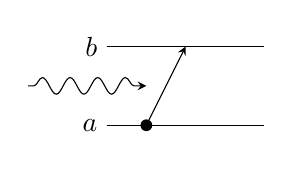
\begin{tikzpicture}
\draw[] (0,0.5) node[left]{$b$} --++ (2,0);
\draw[] (0,-0.5) node[left]{$a$} --++ (2,0);
\draw[-stealth] (0.5,-0.5) node[fill=black,circle,inner sep=1.5pt]{} -- (1,0.5);
\draw[-stealth,decorate,decoration={snake,amplitude=3pt,pre length=2pt,post length=3pt}] (-1,0) --++ (1.5,0);
\end{tikzpicture}
\caption{جذب}
\end{subfigure}\hfill
\begin{subfigure}{0.3\textwidth}
\centering
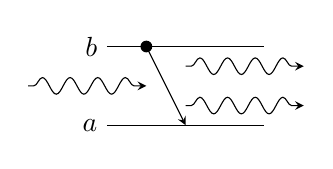
\begin{tikzpicture}
\draw[] (0,0.5) node[left]{$b$} --++ (2,0);
\draw[] (0,-0.5) node[left]{$a$} --++ (2,0);
\draw[-stealth] (0.5,0.5) node[fill=black,circle,inner sep=1.5pt]{} -- (1,-0.5);
\draw[-stealth,decorate,decoration={snake,amplitude=3pt,pre length=2pt,post length=3pt}] (-1,0) --++ (1.5,0);
\draw[-stealth,decorate,decoration={snake,amplitude=3pt,pre length=2pt,post length=3pt}] (1,0.25) --++ (1.5,0);
\draw[-stealth,decorate,decoration={snake,amplitude=3pt,pre length=2pt,post length=3pt}] (1,-0.25) --++ (1.5,0);
\end{tikzpicture}
\caption{تحرک زدہ اخراج}
\end{subfigure}\hfill
\begin{subfigure}{0.3\textwidth}
\centering
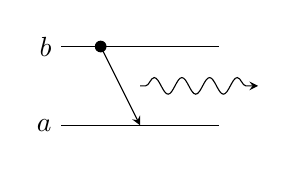
\begin{tikzpicture}
\draw[] (0,0.5) node[left]{$b$} --++ (2,0);
\draw[] (0,-0.5) node[left]{$a$} --++ (2,0);
\draw[-stealth] (0.5,0.5) node[fill=black,circle,inner sep=1.5pt]{} -- (1,-0.5);
\draw[-stealth,decorate,decoration={snake,amplitude=3pt,pre length=2pt,post length=3pt}] (1,0) --++ (1.5,0);
\end{tikzpicture}
\caption{ازخود اخراج}
\end{subfigure}
\caption{روشنی کا جوہر کے ساتھ تین قسم کے باہم عمل پائے جاتے ہیں۔ }
\label{شکل_تابع_وقت_احتمال_روشنی_باہم_عمل}
\end{figure}


اس عمل میں برقناطیسی میدان سے جوہر \عددی{E_b - E_a = \hslash\omega_0} توانائی جذب کرتا ہے۔ ہم کہتے ہیں اس نے \قول{ ایک نوریہ جذب کیا} (شکل \حوالہ{شکل_تابع_وقت_احتمال_روشنی_باہم_عمل}-ا)۔ ( جیسا میں ذکر کر چکا ہوں، لفظ \قول{ نوریہ} در حقیقت \اصطلاح{ کوانٹائی برقی حرکیات}\فرہنگ{کوانٹائی برقی حرکیات}\حاشیہب{quantum electrodynamics}\فرہنگ{quantum electrodynamics}[ برقناطیسی میدان کی کوانٹائی نظریہ] سے تعلق رکھتا ہے، جبکہ ہم میدان کو کلاسیکی نقطہ نظر سے دیکھ رہے ہیں۔ یہ زبان اُس وقت تک استعمال کرنا مناسب ہے جب تک آپ اس سے زیادہ گہرے مطلب نہ لیں۔)

یقیناً، میں بالا حال ( \عددی{(c_a(0)=0)} اور \عددی{(c_b(0)=1)}) سے آغاز کرتے ہوئے پورا عمل دوبارہ کر سکتا ہوں۔ آپ چاہیں تو ایسا کر سکتے ہیں؛ نتیجہ بالکل وہی ہو گا؛ البتہ اس
 مرتبہ \عددی{P_{b\to a} = |c_a(t)|^2} حاصل ہوگا، جو نیچے زیریں سطح میں تحویل کا احتمال ہوگا۔
\begin{align}\label{مساوات_تابع_مضطرب_تحویلی_احتمال_سعت}
	P_{b\to a} (t) = \Big(\frac{\abs{\wp}E_0}{\hslash}\Big)^2 \frac{\sin^2[(\omega_0 - \omega)t/2]}{(\omega_0 - \omega)^2}
\end{align}
(چونکہ ہم \عددی{a} اور \عددی{b} کو آپس میں بدل \عددی{(a\leftrightarrow b)} رہے ہیں جو \عددی{\omega_0} کی جگہ \عددی{-\omega_0} ڈالتا ہے، لہٰذا لازماً یہی نتیجہ حاصل ہوگا۔ مساوات \حوالہ{مساوات_تابع_مضطرب_دو_اجزاء} پر پہنچ کر اب ہم پہلا جزو چنتے ہیں جس کے نسب نما میں \عددی{-\omega_0 + \omega} ہو گا، باقی حساب پہلے کی طرح ہے۔) لیکن اگر آپ رک کر سوچیں تو یہ ایک حیرت انگیز نتیجہ ہے: بالا حال میں پائے جانے والے ذرے پر روشنی کی شعاع ڈالنے سے ذرہ زیریں حال میں تحویل ہوتا ہے اور اس کا احتمال بالکل ٹھیک وہی ہوگا جو زیریں حال سے بالا حال تحویل کا ہے۔ اس عمل کو \اصطلاح{ تحرک زدہ اخراج}\فرہنگ{تحرک زدہ اخراج}\حاشیہب{stimulated emission}\فرہنگ{stimulated emission} کہتے ہیں، جس کی پیشنگوئی آئنشٹائن نے کی تھی۔

تحرک زدہ اخراج کی صورت میں برقناطیسی میدان جوہر سے \عددی{\hslash\omega_0} توانائی کرتا ہے؛ ہم کہتے ہیں ایک نوریہ داخل ہوا اور دو نوریے ( ایک اصل جس نے تحویل پیدا کی اور دوسرا جو تحویل کی بدولت پیدا ہوا) باہر نکلے (شکل \حوالہ{شکل_تابع_وقت_احتمال_روشنی_باہم_عمل}-ب)۔اس طرح \اصطلاح{افزائش}\فرہنگ{افزائش}\حاشیہب{amplification}\فرہنگ{amplification} کا امکان پیدا ہوتا ہے، چونکہ ایک بوتل میں بہت سارے جوہر، جو بالا حال میں ہوں، کو ایک آمدی نوریہ \اصطلاح{ متحرک }\فرہنگ{متحرک}\حاشیہب{trigger}\فرہنگ{trigger} کر کے \اصطلاح{ مسلسل تعامل}\فرہنگ{مسلسل تعامل}\حاشیہب{chain reaction}\فرہنگ{chain reaction} پیدا کریگا؛ یوں پہلا نوریہ \عددی{2} نوریے پیدا کرے گا، یہ نوریے \عددی{4} پیدا کریں گے، وغیرہ۔\اصطلاح{ لیزر}\فرہنگ{لیزر}\حاشیہب{laser}\فرہنگ{laser} کا اصول یہی ہے۔ دھیان رہے کہ ( لیزر عمل کے لیے) ضروری ہے کہ جوہر کی اکثریت بالا حال میں پہنچائی جائے ( جسے \اصطلاح{ آبادی الٹنا}\فرہنگ{آبادی الٹنا}\حاشیہب{population inversion}\فرہنگ{population inversion} کہتے ہیں)؛ چونکہ انجذاب ( جو ایک نوریہ کم کرتا ہے) اور تحرک زدہ اخراج (جو ایک پیدا کرتا ہے) بالمقابل ہوں گے، لہٰذا دونوں حالات کی برابر تعداد سے آغاز کر کے افزائش پیدا نہیں کی جا سکتی۔ 

(انجذاب اور تحرک شدہ اخراج کے علاوہ) روشنی اور مادے کے باہم عمل کا تیسرا طریقہ بھی پایا جاتا ہے؛ اس کو \اصطلاح{ ازخود اخراج}\فرہنگ{ازخود اخراج}\حاشیہب{spontaneous emission}\فرہنگ{spontaneous emission} کہتے ہیں۔ اس میں بیرونی برقناطیسی میدان، جو اخراج پیدا کر سکتا تھا، کی عدم موجودگی میں ہیجان جوہر زیریں حال میں تحویل ہو کر ایک نوریہ خارج کرتا ہے (شکل \حوالہ{شکل_تابع_وقت_احتمال_روشنی_باہم_عمل}-ج)۔ 	ہیجان حال سے جوہر کا زمینی حال میں تنزل عموماً اسی ذریعہ سے ہوتا ہے۔ پہلی نظر میں واضح نہیں کہ ازخود اخراج کیوں کر ہو گا۔ ساکن حال (اگرچہ ہیجان) جوہر کو کیا ضرورت پیش آتی ہے کہ وہ بیرونی اضطراب کی عدم موجودگی میں زمینی حال میں تحویل ہو، اسے وہیں عمر بھر رہنا چاہیے۔ درحقیقت، جوہر وہیں رہتا اگر اس پر کسی قسم کا بیرونی اضطراب اثر انداز نہ ہوتا۔ البتہ، کوانٹائی برقی حرکیات میں زمینی حال میں بھی میدان غیر صفر نہیں ہوتے؛ جیسا ( مثال کے طور پر) ہارمونی مرتعش زمینی حال میں بھی غیر صفر توانائی \عددی{(\hslash\omega/2)} کا حامل ہے۔ آپ تمام روشنی کو روک لیں، کمرے کو مطلق صفر حرارت پر لے جائیں، تب بھی کچھ برقناطیسی شعاع پائی جائے گی، اور یہی \قول{ صفر نقطی} اخراج ازخود اخراج کا سبب بنتا ہے۔ اگر جڑ سے دیکھا جائے تو تمام اخراج تحرک شدہ اخراج ہوگا۔ آپ کو یہ امتیاز کرنا ہو گا کہ آیا آپ میدان فراہم کر رہے ہیں یا قدرتی میدان پایا جاتا ہے۔ اس نقطہ نظر سے یہ کلاسیکی اخراجی عمل کے بالکل اُلٹ ہے، جہاں تمام اخراج ازخود ہوتا ہے اور تحرک شدہ اخراج کا تصور نہیں پایا جاتا۔

کوانٹائی برقی حرکیات اس کتاب کی دسترس سے باہر ہے،\حاشیہد{آئنشٹائن کا مقالہ مساوات شروڈنگر کی آمد سے قبل \سن{1917} میں شائع ہوا۔ اس دلیل میں پلانک سیاہ جسمی کلیہ (مساوات \حوالہ{مساوات_متماثل_سیاہ_جسمی_طیف})، جو \سن{1900} میں منظر عام پر آیا، کے ذریعہ کوانٹائی حرکیات داخل ہوتی ہے۔} تاہم آئنشٹائن کی ایک خوبصورت دلیل ان تینوں (انجذاب، تحرک شدہ اخراج اور ازخود اخراج) کا تعلق پیش کرتی ہے۔ آئنشٹائن نے ازخود اخراج کی وجہ ( زمینی حال برقناطیسی میدان کا اضطراب) پیش نہیں کی، تاہم انکے نتائج ہمیں ازخود اخراج کا حساب کرنے کا مجاز بناتی ہے، جس سے ہیجان جوہری حال کا قدرتی عرصہ حیات تلاش کیا جا سکتا ہے۔\حاشیہد{متبادل اشتقاق کے لئے سوال \حوالہ{سوال_تابع_مضطرب_متبادل_اشتقاق} دیکھیں۔} البتہ ایسا کرنے سے پہلے، ہر طرف سے غیر یک رنگی، غیر تقطیب شدہ، غیر اتساقی برقناطیسی امواج کی آمد (جیسا حقیقت میں ہو گا) سے جوہر کے رد عمل پر بات کرتے ہیں؛ حراری شعاع میں جوہر رکھنے سے ایسی صورتحال پیدا ہوگی۔

\جزوحصہ{غیر اتساقی اضطراب}\شناخت{حصہ_تابع_مضطرب_غیر_اتساقی_اضطراب}
برقناطیسی موج کی کثافت توانائی درج ذیل ہے، جہاں \عددی{E_0} ہمیشہ کی طرح برقی میدان کا حیطہ ہے۔\حاشیہد{برقناطیسی میدان میں فی اکائی حجم توانائی درج ذیل ہے۔
\begin{align*}
u=(\epsilon_2/2)E^2+(1/2\mu_0)B^2
\end{align*}
برقناطیسی موج کے لئے برقی اور مقناطیسی حصے برابر ہوں گے، لہٰذا
\begin{align*}
u=\epsilon_0E^2=\epsilon_0 E_0^2\cos^2(\omega t)
\end{align*}
ہو گا، اور چونکہ \عددی{\cos^2} (یا \عددی{\sin^2}) کا اوسط \عددی{1/2} ہے لہٰذا ایک مکمل پھیرے پر اوسط \عددی{(\epsilon_0/2)E_0^2} ہو گا۔}
\begin{align}
	u = \frac{\epsilon_0}{2}E^2_0
\end{align}
یوں حیرانی کی بات نہیں کہ تحویلی احتمال (مساوات \حوالہ{مساوات_تابع_مضطرب_تحویلی_احتمال_سعت}) میدان کی کثافت توانائی کا راست متناسب ہے۔
\begin{align}
	P_{b\to a }(t) = \frac{2u}{\epsilon_0\hslash^2}\abs{\wp}^2 \frac{\sin^2[(\omega_0-\omega)t/2]}{(\omega_0-\omega)^2}
\end{align}
تاہم یہ نتیجہ واحد ایک تعدد \عددی{\omega} پر \اصطلاح{یک رنگی}\فرہنگ{یک رنگی}\حاشیہب{monochromatic}\فرہنگ{monochromatic} موج کے لیے درست ہوگا۔ عملی استعمال کے کئی نظاموں پر وسیع تعددی سعت کی برقناطیسی امواج کی روشنی ڈالی جاتی ہے۔ ایسی صورت میں \عددی{u\to\rho(\omega)\dif \omega} ہوگا، جہاں \عددی{\rho(\omega)\dif \omega} تعددی سعت \عددی{\dif\omega} میں کثافت توانائی ہے، اور خالص تحویلی احتمال درج ذیل تکمل کا روپ اختیار کرے گا۔\حاشیہد{مساوات \حوالہ{مساوات_تابع_مضطرب_تکمل_روپ} فرض کرتی ہے کہ مختلف تعدد پر تحویل ایک دوسرے کے غیر تابع ہیں، لہٰذا کل تحویلی احتمال ان انفرادی احتمالات کا مجموعہ ہو گا۔ اگر مختلف حصے \اصطلاح{اتساقی}\فرہنگ{اتساقی} ہوں، تب ہمیں حیطوں \عددی{(c_b(t))} نہ کہ احتمالات \عددی{(|c_b(t)|^2)} کا مجموعہ لینا ہو گا، اور اس میں حیطوں کے مربعوں کے علاوہ حاصل ضرب بھی پائے جائیں گے۔ ہم عملی استعمال میں ہر مرتبہ فرض کرتے ہیں کہ اضطراب غیر اتساقی ہے۔}
\begin{align}\label{مساوات_تابع_مضطرب_تکمل_روپ}
	P_{b\to a}(t) = \frac{2}{\epsilon_0\hslash^2}\abs{\wp}^2\int_{0}^{\infty}\rho(\omega){\frac{\sin^2[(\omega_0-\omega)t/2]}{(\omega_0-\omega)^2}}\dif \omega
\end{align}

لہریا قوسین میں جزو کی \عددی{\omega_0} پر نوکدار چوٹی پائی جاتی ہے (شکل \حوالہ{شکل_تابع_وقت_احتمال_جبری_تعدد})، جبکہ عام طور پر \عددی{\rho(\omega)} کافی چوڑا ہوگا، لہٰذا ہم \عددی{\rho\omega} کی جگہ \عددی{\rho(\omega_0)} لکھ کر اسے تکمل کے باہر منتقل کر سکتے ہیں۔
\begin{align}
	P_{b\to a}(t) \cong \frac{2\abs{\wp}^2}{\epsilon_0\hslash^2}\rho(\omega_0)\int_{0}^{\infty}\frac{\sin^2[(\omega_0-\omega)t/2]}{(\omega_0-\omega)^2}\dif \omega
\end{align}
متغیرات کو تبدیل کر کے \عددی{x\equiv(\omega_0-\omega)t/2} لکھ کر (اور چونکہ بنیادی طور پر متکمل باہر صفر ہی ہے) تکمل کی حدوں کو \عددی{x = \pm\infty} تک وسعت دے کر، اور قطعی تکمل کو جدول سے دیکھ کر:
\begin{align}
	\int_{-\infty}^{\infty}\frac{\sin^2x}{x^2}\dif x = \pi
\end{align}
درج ذیل حاصل ہوتا ہے۔
\begin{align}\label{مساوات_تابع_مضطرب_متناسب_وقت}
	P_{b\to a}(t)\cong\frac{\pi\abs{\wp}^2}{\epsilon_0\hslash^2}\rho(\omega_0)t
\end{align}
اس مرتبہ تحویلی احتمال \عددی{t} کا راست متناسب ہے۔ آپ نے دیکھا کہ یک رنگی اضطراب کے برعکس، غیر اتساقی وسیع تعدد کی شعاع پلٹیں کھاتا ہوا احتمال نہیں دیتی۔ بالخصوص، \اصطلاح{تحویلی شرح}\فرہنگ{تحویلی شرح}\حاشیہب{transition rate}\فرہنگ{transition rate} \عددی{(R\equiv \dif P/\dif t)} اب ایک مستقل ہوگا۔
\begin{align}
	R_{b\to a}& = \frac{\pi}{\epsilon_0\hslash^2}\abs{\wp}^2\rho(\omega_0)&&\text{\small\RL{(مستقل تحویلی شرح)}}
\end{align}


اب تک ہم فرض کرتے رہے ہیں کہ اضطرابی موج \عددی{y} رخ سے آمدی (شکل \حوالہ{شکل_تابع_وقت_احتمال_برقناطیسی_موج}) اور \عددی{z} رخ تقطیب شدہ ہے۔ لیکن ہم اُس صورت میں دلچسپی رکھتے ہیں جب جوہر پر شعاع ہر رخ سے آمدی ہو، اور اس میں ہر ممکنہ تقطیب پائی جاتی ہو؛ میدان کی توانائی \عددی{(\rho(\omega))} ان مختلف انداز میں برابر تقسیم ہوگی۔ ہمیں \عددی{|\wp|^2} کے بجائے \عددی{\abs{\kvec{\wp}\cdot \kvecsub{a}{n}}^2} کی اوسط قیمت درکار ہوگی، جہاں (مساوات \حوالہ{مساوات_تابع_مضطرب_وابستگی} کو عمومیت دیتے ہوئے) درج ذیل ہوگا،
\begin{align}\label{مساوات_تابع_مضطرب_ٹیڑا_پی}
	\kvec{\wp} \equiv q \langle \psi_b|\kvec{r}|\psi_a \rangle
\end{align}
اور اوسط تمام تقطیب اور تمام آمدی رخ پر لیا جائے گا۔
\begin{figure}
\centering
\begin{tikzpicture}
\draw[-stealth,name path=px] (0,0) -- ++(-135:2.5) coordinate(kx) node[left]{$x$};
\draw[-stealth,name path=py] (0,0) --++ (0:4) coordinate(ky) node[below]{$y$};
\draw[-stealth,name path=pz] (0,0) -- ++(90:2) coordinate(kz) node[left]{$z$};
\draw[thick,-latex] (0,0)--++(-70:1.5) coordinate(kn) node[pos=0.5,right]{$\kvecsub{a}{n}$};
\draw[thick,-latex] (0,0)--++(20:3) coordinate(kp) node[pos=0.7,below right]{$\kvec{\wp}$};
\draw[] ([shift={(-135:0.5)}]0,0) arc (-135:-70:0.5) node[pos=0.5,below]{$\phi$};
\draw[] ([shift={(20:0.5)}]0,0) arc (20:90:0.5) node[pos=0.5,above]{$\theta$};
\path[name path=pn](kn)--++(-2,0);
\draw[dashed,name intersections={of={pn and px}}] (kn)--(intersection-1);
\path[name path=pp](kp)--++(-3,0);
\draw[dashed,name intersections={of={pp and pz}}] (kp)--(intersection-1);
\path[name path=ppp](kp)--++(0,-2);
\draw[dashed,name intersections={of={ppp and py}}] (kp)--(intersection-1);
\end{tikzpicture}
\caption{محدد برائے \عددی{\abs{\kvec{\wp}\cdot\kvecsub{a}{n}}^2} کی اوسط زنی۔}
\label{شکل_تابع_وقت_اوسط_زنی_محدد}
\end{figure}


 اوسط درج ذیل طریقہ سے حاصل کیا جا سکتا ہے: کروی محدد یوں منتخب کریں کہ شعاع کی حرکت کا رخ \عددی{z} محور پر ہو (تاکہ تقطیب \عددی{xy} سطح میں ہو) اور (اٹل) سمتیہ \عددی{ \kvec{p}} سطح \عددی{yz} میں پایا جاتا ہو (شکل \حوالہ{شکل_تابع_وقت_اوسط_زنی_محدد})۔\حاشیہد{میں \عددی{\kvec{\wp}} کو حقیقی کی طرح تصور کرتا ہوں، اگرچہ یہ عموماً مخلوط ہو گا۔ درج ذیل کی بنا پر
 \begin{align*}
 |\kvec{\wp}\cdot\kvecsub{a}{n}|^2=|(\kvec{\wp}_{\text{حقیقی}})\cdot\kvecsub{a}{n}+i(\kvec{\wp}_{\text{خیالی}})\cdot\kvecsub{a}{n}|^2=|(\kvec{\wp}_{\text{حقیقی}})\cdot\kvecsub{a}{n}|^2+|(\kvec{\wp}_{\text{خیالی}})\cdot\kvecsub{a}{n}|^2
 \end{align*}
 ہم حقیقی اور خیالی حصوں کا حساب علیحدہ علیحدہ کر کے نتائج جمع کر سکتے ہیں۔ مساوات \حوالہ{مساوات_تابع_مضطرب_شرح_بی_تا_اے} میں مطلق قیمت علامت دو کام کر رہی ہے، یہ سمتیہ کی مقدار اور مخلوط حیطہ:
 \begin{align*}
 |\kvec{\wp}|^2=|\wp_x|^2+|\wp_y|^2+|\wp_z|^2
 \end{align*}
 ظاہر کرتی ہے۔
 }
\begin{align}
	\kvecsub{a}{n} &= \cos\phi\ai+\sin\phi\aj, && \kvec{\wp}=\wp\sin\theta\aj+\wp\cos\theta\ak
\end{align} 
تب 
\begin{align*}
\kvec{\wp}\cdot\kvecsub{a}{n}=\wp\sin\theta\sin\phi
\end{align*}
اور درج ذیل ہوگا۔ 
\begin{align}
	\abs{\kvec{\wp}\cdot \kvecsub{a}{n}}^2_{\text{\RL{اوسط}}} &= \frac{1}{4\pi}\int\abs{\kvec{\wp}}^2\sin^2\theta\sin^2\phi \dif \theta \dif \phi\nonumber\\
 &= \frac{\abs{\kvec{\wp}}^2}{4\pi}\int_0^{\pi}\sin^3\theta\dif\theta\int_0^{2\pi}\sin^2\phi\dif\phi = \frac{1}{3}\abs{\kvec{\wp}}^2
\end{align}
\ترچھا{ماخوذ:} ہر جانب سے آمدی، غیر تقطیبی، غیر اتساقی شعاع کے زیر اثر حال \عددی{b} سے حال \عددی{a} میں تحرک شدہ اخراج کی تحویلی شرح درج ذیل ہوگی،
\begin{align}\label{مساوات_تابع_مضطرب_شرح_بی_تا_اے}
	R_{b\to a} = \frac{\pi}{3\epsilon_0\hslash^2}\abs{\kvec{\wp}}^2\rho(\omega_0)
\end{align}
جہاں دو حالات کے بیچ برقی جفت قطب معیار اثر کا قالبی رکن \عددی{\kvec{\wp}} ہوگا (مساوات \حوالہ{مساوات_تابع_مضطرب_ٹیڑا_پی}) اور \عددی{\omega_0 = (E_b-E_a)/\hslash} پر فی اکائی تعدد میدان میں کثافت توانائی \عددی{\rho(\omega_0)} ہوگی۔\حاشیہد{یہ تابع وقت نظریہ اضطراب کے \اصطلاح{ فرمی کے سنہرا قانون}\فرہنگ{فرمی!سنہرا قانون}\فرہنگ{Fermi's Golden rule} کی ایک مخصوص صورت ہے، جو کہتا ہے کہ تحویلی شرح، اضطرابی مخفیہ کے قالبی ارکان کے مربع اور تحویلی تعدد پر اضطراب کے زور کا راست متناسب ہو گا۔}

%==============

\حصہ{ازخود اخراج}
\جزوحصہ{آئنشٹائن عددی سر \عددی{A} اور \عددی{B}}
فرض کریں ایک برتن میں زیریں حال \عددی{\psi_a} میں \عددی{N_a} اور بالا حال \عددی{\psi_b} میں \عددی{N_b} جوہر پائے جاتے ہوں۔ ازخود اخراجی شرح کو \عددی{A} لیتے ہوئے،\حاشیہد{میں عام طور پر تحویلی شرح کے لئے علامت \عددی{R} استعمال کرتا ہوں، لیکن اس سیاق و سباق میں، باقی لوگوں کی طرح، میں بھی آئنشٹائن کی علامتیت استعمال کروں گا۔} اکائی وقت میں بالا حال سے \عددی{N_bA} ذرات ازخود عمل کے ذریعہ نکلیں گے۔\حاشیہد{ذرات کی تعداد \عددی{N_a} اور \عددی{N_b}بہت بڑی تصور کریں، لہٰذا ہم انہیں وقت کے استمراری تفاعلات تصور کر کے شماریاتی اتار چھڑاو نظر انداز کرتے ہیں۔} جیسا ہم (مساوات \حوالہ{مساوات_تابع_مضطرب_شرح_بی_تا_اے}) دیکھ چکے ہیں تحرک شدہ اخراج کی تحویلی شرح برقناطیسی میدان کی کثافت توانائی، \عددی{B_{ab}\rho(\omega_0)}، کے راست متناسب ہوگی؛ یوں بالا حال سے تحرک شدہ اخراج کی بنا پر اکائی وقت میں \عددی{N_bB_{ba}\rho(\omega_0)} ذرات نکلیں گے۔ اسی طرح انجذابی شرح \عددی{\rho(\omega_0)} کی راست متناسب ہے، جسے ہم \عددی{B_{ab}\rho(\omega_0)} کہتے ہیں؛ لہٰذا اکائی وقت میں \عددی{N_aB_{ab}\rho(\omega_0)} ذرات بالا حال میں شامل ہوں گے۔ ان تمام کو یکجا کر کے درج ذیل حاصل ہو گا۔
\begin{align}
	\frac{\dif N_b}{\dif t} = -N_bA-N_bB_{ba}\rho(\omega_0)+N_aB_{ab}\rho(\omega_0)
\end{align}

فرض کریں یہ جوہر محیط میدان کے ساتھ حراری توازن میں ہیں، لہٰذا ہر سطح میں ذرات کی تعداد مستقل ہوگی۔یوں \عددی{\dif N_b/\dif t = 0} لہٰذا درج ذیل ہو گا۔
\begin{align}
	\rho(\omega_0) = \frac{A}{(N_a/N_b)B_{ab}-B_{ba}}
\end{align}
ہم بنیادی شماریاتی میکانیات سے جانتے ہیں کہ، درجہ حرارت \عددی{T} پر حراری توازن میں، توانائی \عددی{E} کے حامل ذرات، کی تعداد \اصطلاح{بولٹزمن جزو ضربی}\فرہنگ{بولٹزمن جزو ضربی}\حاشیہب{Boltzmann factor}\فرہنگ{Boltzmann factor} \عددی{e^{(-E/k_BT)}} کے راست متناسب ہوگی؛ یوں
\begin{align}
	\frac{N_a}{N_b} = \frac{e^{-E_a/k_{B}T}}{e^{-E_b/k_BT}} = e^{\hslash\omega_0/k_BT}
\end{align}
لہٰذا درج ذیل ہو گا۔
\begin{align}
	\rho(\omega_0) = \frac{A}{e^{\hslash\omega_0/k_BT}B_{ab}-B_{ba}}
\end{align}

لیکن پلانک کا سیاہ جسمی کلیہ (مساوات \حوالہ{مساوات_متماثل_سیاہ_جسمی_طیف}) ہمیں حراری شعاع کی کثافت توانائی دیتی ہے۔
\begin{align}
	\rho(\omega) = \frac{\hslash}{\pi^2c^3}\frac{\omega^3}{e^{\hslash\omega/k_BT}-1}
\end{align}
ان دونوں ریاضی فقروں کا موازنہ کرنے سے 
\begin{align}\label{مساوات_تابع_مضطرب_برابر_شرح}
	B_{ab} = B_{ba}
\end{align}
اور درج ذیل حاصل ہوگا۔
\begin{align}\label{مساوات_تابع_مضطرب_شرح_خود_با_خود_اخراج}
	A = \frac{\omega^3_0\hslash}{\pi^2c^3}B_{ba}
\end{align}
مساوات \حوالہ{مساوات_تابع_مضطرب_برابر_شرح} اُس بات کی تصدیق کرتی ہے جو ہم پہلے سے جانتے تھے: تحرک شدہ اخراج کی تحویلی شرح وہی ہے جو انجذاب کی ہے۔\سن{1907} میں یہ ایک حیرت کن نتیجہ تھا جس میں آئنشٹائن کو اس بات پر مجبور کیا کہ وہ کلیہ پلانک حاصل کرنے کی خاطر تحرک شدہ اخراج کا تصور پیدا کرے۔ تاہم ہم یہاں مساوات \حوالہ{مساوات_تابع_مضطرب_شرح_خود_با_خود_اخراج} میں دلچسپی رکھتے ہیں، جو ہمیں تحرک شدہ اخراجی شرح \عددی{(B_{ba}\rho(\omega_0))}، جسے ہم پہلے سے جانتے ہیں، کی صورت میں ازخود اخراجی شرح \عددی{(A)} دیتی ہے۔ جسے ہم جاننا چاہتے ہیں مساوات \حوالہ{مساوات_تابع_مضطرب_شرح_بی_تا_اے} سے
\begin{align}
	B_{ba} = \frac{\pi}{3\epsilon_0\hslash^2}\abs{\kvec{\wp}}^2
\end{align}
لیتے ہیں، لہٰذا ازخود اخراجی شرح درج ذیل ہوگی۔
\begin{align}\label{مساوات_تابع_مضطرب_خود_با_خود_شرح_حتمی}
	A = \frac{\omega^3_0\abs{\kvec{\wp}}^2}{3\pi\epsilon_0\hslash c^3}
\end{align}

\ابتدا{سوال}\شناخت{سوال_تابع_مضطرب_متبادل_اشتقاق}
نیچے کی طرف تحویل میں ازخود اخراج اور حراری تحرک شدہ اخراج ( وہ تحرک شدہ اخراج جو سیاہ جسم شعاع کی بنا پر ہو) میں مقابلہ ہوتا ہے۔ دکھائیں کہ رہائشی درجہ حرارت \عددی{(T = \SI{300}{\kelvin})} پر \عددی{\SI{5e12}{\hertz}} سے بہت کم تعددوں پر حراری تحرک شدہ اخراج غالب ہوگا، جبکہ \عددی{\SI{5e12}{\hertz}} سے بہت زیادہ تعددوں پر ازخود اخراج غالب ہوگا۔ بصری روشنی کے لیے کونسا غالب ہوگا؟
\انتہا{سوال}
\ابتدا{سوال}
برقناطیسی میدان کی زمینی حال کثافت توانائی \عددی{\rho_0(\omega)} جانتے ہوئے ازخود اخراجی شرح درحقیقت تحرک شدہ اخراجی شرح (مساوات \حوالہ{مساوات_تابع_مضطرب_شرح_بی_تا_اے}) ہوگی، لہٰذا آئنشٹائن عددی سر \عددی{A} اور \عددی{B} جانے بغیر آپ ازخود اخراجی شرح (مساوات \حوالہ{مساوات_تابع_مضطرب_خود_با_خود_شرح_حتمی}) اخذ کر سکتے ہیں۔ اگرچہ ایسا کرنے کے لیے کوانٹائی برقی حرکیات بروئے کار لانی ہوگی، تاہم اگر آپ یہ قبول کریں کہ زمینی حال میں \ترچھا{ ایک نوریہ فی انداز} پایا جاتا ہے، تب اس کو اخذ کرنا بہت آسان ہوگا:
\begin{enumerate}[a.]
\item
مساوات \حوالہ{مساوات_مماثل_عدد_مکین} کی جگہ \عددی{N_\omega = d_k} پُر کرکے \عددی{\rho_0(\omega)} اخذ کریں ( زیادہ تعدد پر اس کلیہ کو ناکارہ ہونا ہوگا ورنہ کل \قول{خلائی توانائی} لامتناہی ہوگی؛ تاہم یہ کہانی کسی دوسرے دن کے لیے چھوڑتے ہیں)۔
\item
 اپنے نتیجہ کے ساتھ مساوات \حوالہ{مساوات_تابع_مضطرب_شرح_بی_تا_اے} استعمال کرکے ازخود اخراجی شرح حاصل کریں۔ مساوات \حوالہ{مساوات_تابع_مضطرب_خود_با_خود_شرح_حتمی} کے
 ساتھ موازنہ کریں۔
 \end{enumerate}
\انتہا{سوال}

%==================================

\جزوحصہ{ہیجان حال کا عرصہ حیات}
مساوات \حوالہ{مساوات_تابع_مضطرب_خود_با_خود_شرح_حتمی} ہمارا بنیادی نتیجہ ہے: یہ تحرک شدہ اخراج کی تحویلی شرح دیتا ہے۔ اب فرض کریں کسی طرح آپ بہت بڑی تعداد میں جوہر کو ہیجان حال منتقل کرتے ہیں۔ از خود اخراج کے نتیجے میں، وقت کے ساتھ یہ تعداد گھٹے گی؛ بالخصوص، دورانیہ \عددی{\dif t} میں جوہروں کی تعداد میں \عددی{A\dif t} کمی ہوگی:
\begin{align}
	\dif N_b = -AN_b\dif t
\end{align}
(جہاں ہم فرض کرتے ہیں کہ مزید جوہر ہیجان انگیز نہیں کیے جا رہے ہیں)۔\حاشیہد{یہ حراری توازن نہیں ہے جس پر گزشتہ حصے میں بات کی گئی۔ یہاں ہم فرض کر رہے ہیں کہ جوہروں کو ہیجان حال میں اٹھایا گیا ہے اور یہ اب واپس توازنی سطحوں کو لوٹ رہے ہیں۔ } اس کو \عددی{N_b(t)} کے لیے حل کرتے ہیں:
\begin{align}
	N_b(t) = N_b(0)e^{-At}
\end{align}
بظاہر، ہیجان حال میں تعداد، قوت نمائی طور پر وقتی مستقل:
\begin{align}
	\tau &= \frac{1}{A}&&\text{\small\RL{(عرصہ حیات)}}
\end{align}
کے ساتھ کم ہو گی، جسے اس حال کا \اصطلاح{عرصہ حیات}\فرہنگ{عرصہ حیات}\حاشیہب{lifetime}\فرہنگ{lifetime} کہتے ہیں۔ ایک عرصہ حیات میں \عددی{N_b(t)} کی قیمت ابتدائی قیمت کی \عددی{1/e \approx \num{0.368}} گنّا ہوگی۔

میں اب تک فرض کرتا آ رہا ہوں کہ نظام میں صرف دو حالات پائے جاتے ہیں، تاہم علامتیت سادہ رکھنے کی خاطر ایسا کیا گیا؛تحرک شدہ اخراج کا کلیہ ( مساوات \حوالہ{مساوات_تابع_مضطرب_خود_با_خود_شرح_حتمی})، دیگر قابل رسائی حالات سے قطع نظر، \عددی{\psi_b \to \psi_a} کی تحویلی شرح دیتا ہے ( سوال \حوالہ{سوال_تابع_مضطرب_دیگر_قطع_نظر} دیکھیں)۔ عمومی طور پر ایک ہیجان جوہر کے کئی مختلف \اصطلاح{ انداز تنزل}\فرہنگ{انداز تنزل}\حاشیہب{decay modes}\فرہنگ{decay modes} ہوں گے ( یعنی: \عددی{\psi_b} کا تنزل بہت سارے زیریں توانائی حالات
 \عددی{\psi_{a1}}، \عددی{\psi_{a2}}، \عددی{\psi_{a3}}، وغیرہ میں ہو سکتا ہے)۔ ایسی صورت میں تمام تحویلی شرحیں جمع ہو کر درج ذیل خالص عرصہ حیات دیں گی۔
\begin{align}
	\tau = \frac{1}{A_1+A_2+A_3+\dotsb}
\end{align}


\ابتدا{مثال}
فرض کریں ایک اسپرنگ کے ساتھ باندھا ہوا بار \عددی{q} محور \عددی{x} پر ارتعاش کا پابند ہے۔ فرض کریں یہ حال \عددی{| n \rangle} (مساوات\حوالہ{مساوات_شروڈنگر_ہارمونی_ساکن_حالات}) سے آغاز کر کے ازخود اخراج کے ذریعے حال \عددی{| n'\rangle} کو پہنچتا ہے۔ مساوات \حوالہ{مساوات_تابع_مضطرب_ٹیڑا_پی}کے تحت درج ذیل ہوگا۔
\begin{align*}
	\kvec{\wp} = q\langle n|x|n'\rangle\ai
\end{align*}
آپ نے سوال \حوالہ{سوال_قواعد_قالبی_ارکان} میں \عددی{x} کے قالبی ارکان:
\begin{align*}
	\langle n|x|n'\rangle = \sqrt{\frac{\hslash}{2m\omega}}(\sqrt{n'}\delta_{n,n'-1}+\sqrt{n}\delta_{n',n-1})
\end{align*}
 تلاش کئے، جہاں مرتعش کا قدرتی تعدد \عددی{\omega} ہے۔ (مجھے تحرک شدہ اخراج کے تعدد کے لیے اس حرف کی ضرورت اب پیش نہیں آئے گی۔) ہم اخراج کی بات کر رہے ہیں لہٰذا \عددی{n'} لازماً \عددی{n} سے نیچے ہوگا؛ یوں ہمارے اس مقصد کے لئے درج ذیل ہوگا۔
\begin{align}
	\kvec{\wp} = q\sqrt{\frac{n\hslash}{2m\omega}}\delta_{n', n-1}\,\ai
\end{align}
بظاہر \قول{سیڑھی} پر صرف ایک پایہ نیچے تحویل ممکن ہے \عددی{(n-n'=1)}؛ اور اخراجی نوریہ کا تعدد درج ذیل ہے۔
\begin{align}
	\omega_0 = \frac{E_n-E_n'}{\hslash} = \frac{(n+1/2)\hslash\omega - (n'+ 1/2)\hslash\omega}{\hslash} =(n-n')\omega = \omega
\end{align}
کوئی حیرانی کی بات نہیں، نظام کلاسیکی ارتعاشی تعدد پر شعاع ریز ہے۔ تحویلی شرح (مساوات \حوالہ{مساوات_تابع_مضطرب_خود_با_خود_شرح_حتمی}) درج ذیل
\begin{align}
	A = \frac{nq^2\omega^2}{6\pi\epsilon_0mc^3}
\end{align}
اور \عددی{n}ویں ساکن حال کا عرصہ حیات درج ذیل ہوگا۔
\begin{align}
	\tau_n = \frac{6\pi\epsilon_0mc^3}{nq^2\omega^2}
\end{align}
چونکہ، ہر ایک اخراجی نوریہ \عددی{\hslash\omega} توانائی ساتھ لے جاتا ہے، لہٰذا اشعاعی طاقت \عددی{A\hslash\omega} ہوگی
\begin{align*}
	P = \frac{q^2\omega^2}{6\pi\epsilon_0mc^3}(n\hslash\omega)
\end{align*}
یا، \عددی{n}ویں حال میں مرتعش کی توانائی \عددی{E = (n+1/2)\hslash\omega} لیتے ہوئے درج ذیل ہوگی۔
\begin{align}\label{مساوات_تابع_مضطرب_زمینی_توانائی_رہے_گی}
	P = \frac{q^2\omega^2}{6\pi\epsilon_0mc^3}\big(E-\frac{1}{2}\hslash\omega\big)
\end{align}
(ابتدائی) توانائی \عددی{E} کے کوانٹائی مرتعش کی اوسط اشعاعی طاقت اتنی ہو گی۔

موازنہ کی خاطر اسی طاقت کے \ترچھا{کلاسیکی} مرتعش کی اوسط اشعاعی طاقت کا تعین کرتے ہیں۔ کلاسیکی برقی حرکیات کے تحت مسرع بار \عددی{q} کی اشعاعی طاقت \اصطلاح{کلیہ لارمر}:\فرہنگ{کلیہ لارمر}\حاشیہب{Larmor formula}\فرہنگ{Larmor formula}
\begin{align}
	P = \frac{q^2a^2}{6\pi\epsilon_0c^3}
\end{align}
 دیتا ہے۔ ہارمونی مرتعش \عددی{x(t) = x_0\cos(\omega t)} کا حیطہ \عددی{x_0}، اور اسراع \عددی{a = -x_0\omega^2\cos(\omega t)} ہوگا۔ ایک مکمل پھیرے پر اوسط درج ذیل ہوگا۔
\begin{align*}
	P = \frac{q^2x^2_0\omega^4}{12\pi\epsilon_0c^3}
\end{align*}
لیکن اس مرتعش کی توانائی \عددی{E = (1/2)m\omega^2x_0^2} ہے، لہٰذا \عددی{x_0^2 = 2E/m\omega^2} ہوگا، جس سے درج ذیل لکھا جا سکتا ہے۔
\begin{align}
	P = \frac{q^2\omega^2}{6\pi\epsilon_0mc^3}E
\end{align}
توانائی \عددی{E} کا کلاسیکی مرتعش اوسطاً اتنی اشعاعی طاقت دے گا۔ کلاسیکی حد \عددی{(\hslash\to0)} میں کلاسیکی اور کوانٹائی کلیات آپس میں متفق ہیں؛\حاشیہد{درحقیقت، \عددی{P} کو \ترچھا{ زمین حال سے زائد} توانائی کی صورت میں لکھیں تو دونوں کلیات متماثل ہوں گے۔} البتہ زمینی حال کو کوانٹائی کلیہ
 (مساوات\حوالہ{مساوات_تابع_مضطرب_زمینی_توانائی_رہے_گی}) تحفظ دیتا ہے: اگر \عددی{E = (1/2)\hslash\omega} ہو تب مرتعش شعاع ریز نہیں ہو گا۔
\انتہا{مثال}
\ابتدا{سوال}
ہیجان حال کی \اصطلاح{نصف حیات}\فرہنگ{نصف حیات}\حاشیہب{half-life}\فرہنگ{half-life} \عددی{(t_{1/2})} سے مراد وہ دورانیہ ہے جس میں بڑی تعداد کے جوہروں میں سے نصف تحویل کرتے ہوں۔ نصف حیات \عددی{t_{1/2}} اور (حال کے) \قول{عرصہ حیات} \عددی{\tau} کے بیچ رشتہ تلاش کریں۔
\انتہا{سوال}
\ابتدا{سوال}\شناخت{سوال_تابع_مضطرب_عرصہ_حیات}
ہائیڈروجن کے چاروں \عددی{n=2} حالات کے لیے عرصہ حیات( سیکنڈوں میں) تلاش کریں۔ \ترچھا{ اشارہ:} آپ کو \عددی{\langle \psi_{100}|x|\psi_{200} \rangle}، \عددی{ \langle \psi_{100}|y|\psi_{211} \rangle}، وغیرہ طرز کے قالبی ارکان کی قیمتیں تلاش کرنی ہوں گی۔ یاد رہے کہ
 \عددی{x = r\sin\theta\cos\phi}، \عددی{y = r\sin\theta\sin\phi} اور \عددی{z = r\cos\theta} ہیں۔ ان میں سے زیادہ تر تکملات صفر کے برابر ہیں، لہٰذا حساب شروع کرنے سے پہلے ان پر ایک گہری نظر ضرور ڈالیں۔

\ترچھا{جواب:} سوائے \عددی{\psi_{200}} جو لامتناہی ہے، باقی تمام کے لیے \عددی{\num{1.60}\times10^{-9}} سیکنڈ ہوگا۔
\انتہا{سوال}

%========================


\جزوحصہ{قواعد انتخاب} 
 ازخود اخراجی شرح درج ذیل روپ کے قالبی ارکان معلوم کر کے حاصل کی جا سکتی ہے۔ 
\begin{align*}
	\langle \psi_b|\kvec{r}|\psi_a \rangle
\end{align*}
اگر آپ نے سوال \حوالہ{سوال_تابع_مضطرب_عرصہ_حیات} حل کیا ہو ( اگر حل نہیں کیا، اسی وقت پہلے اس کو حل کریں!) تو آپ نے دیکھا ہوگا کہ یہ مقداریں عموماً \ترچھا{ صفر} ہوتی ہیں، اور کیا بہتر ہوگا اگر ہم پہلے سے جان سکیں کہ کون سے تکملات صفر دیں گے، تاکہ ہم اپنا وقت غیر ضروری تکملات حل کرنے میں ضائع نہ کریں۔ فرض کریں ہم ہائیڈروجن کی طرح کے نظام میں دلچسپی رکھتے ہیں، جس کی ہیملٹنی کروی تشاکلی ہے۔ ایسی صورت میں ہم حالات کو عمومی کوانٹائی اعداد \عددی{n}، \عددی{\ell}، اور \عددی{m} سے ظاہر کر سکتے ہیں اور قالبی ارکان درج ذیل ہوں گے۔ 
\begin{align*}
	\langle n'\ell'm'|\kvec{r}|n\ell m \rangle
\end{align*}
زاویائی معیاری حرکت مقلبیت رشتے اور زاویائی معیاری حرکت عاملین کی ہرمشی پن مل کر اس مقدار پر طاقتور پابندیاں عائد کرتے ہیں۔

\جزوحصہء{انتخابی قواعد برائے \عددی{m} اور \عددی{m'}:}
 ہم پہلے \عددی{x}، \عددی{y}، اور \عددی{z} کے ساتھ \عددی{L_z} کے مقالب پر غور کرتے ہیں جنہیں باب \حوالہ{باب_تین_ابعادی_کوانٹائی_میکانیات} میں حاصل کیا گیا (مساوات \حوالہ{مساوات_تین_ابعادی_مقلبی_رشتے} دیکھیں)۔
\begin{align}
	[L_z, x] = i\hslash y, \quad [L_z, y] = -i\hslash x, \quad [L_z, z] = 0
\end{align}
ان میں تیسرے سے درج ذیل حاصل ہوتا ہے۔
\begin{align*}
	0 &= \langle n'\ell'm'|[L_z, z]|n\ell m \rangle = \langle n'\ell'm'\abs{L_zz - zL_z}n\ell m \rangle \\
	&= \langle n'\ell'm'|[(m'\hslash)z - z(m\hslash)]|n\ell m \rangle = (m'- m)\hslash\langle n'\ell'm'|z|n\ell m \rangle
\end{align*}
\موٹا{ماخوذ:} 
\begin{align}\label{مساوات_تابع_مضطرب_ماخوذ_الف}
 \langle n'\ell'm'|z|n\ell m \rangle = 0 \quad \text{\RL{یا پھر}}\quad m'= m \quad \text{\RL{یا}}
\end{align}
لہٰذا، ما سوائے \عددی{m'= m} کی صورت میں، \عددی{z} کے قالبی ارکان ہر صورت صفر ہوں گے۔

ساتھ ہی، \عددی{x} کے ساتھ \عددی{L_z} کا مقلب درج ذیل دے گا۔
\begin{align*}
	\langle n'\ell 'm'|[L_z, x]|n\ell m \rangle &= \langle n'\ell'm'|(L_zx - xL_z)|n\ell m \rangle \\
	&= (m'- m)\hslash\langle n'\ell'm'|x|n\ell m \rangle = i\hslash\langle n'\ell'm'|y|n\ell m \rangle
\end{align*}
\موٹا{ماخوذ:}
\begin{align}\label{مساوات_تابع_مضطرب_ماخوذ_ب}
	(m'- m)\langle n'\ell'm'|x|n\ell m \rangle = i\langle n'\ell'm'|y|n\ell m \rangle
\end{align}

یوں، آپ \عددی{y} کے قالبی ارکان کو \عددی{x} کے مطابقتی قالبی ارکان سے حاصل کر سکتے ہیں، اور آپ کو کبھی بھی \عددی{y} کے قالبی ارکان کے حساب کی ضرورت پیش نہیں آئے گی۔

اور آخر میں، \عددی{y} کے ساتھ \عددی{L_z} کا مقلب درج ذیل دیتا ہے۔ 
\begin{align*}
	\langle n'\ell'm' |[L_z, y]| n\ell m \rangle &= \langle n'\ell'm' |(L_zy-yL_z) |n\ell m \rangle\\
	&= (m'-m)\hslash\langle n'\ell'm'|y|n\ell m \rangle = -i\hslash\langle n'\ell'm'|x|n\ell m \rangle
\end{align*}
\موٹا{ماخوذ:}
\begin{align}\label{مساوات_تابع_مضطرب_ماخوذ_پ}
	(m'- m)\langle n'\ell'm'|y|n\ell m \rangle = -i\langle n'\ell'm'|x|n\ell m \rangle
\end{align}
بالخصوص، مساوات\حوالہ{مساوات_تابع_مضطرب_ماخوذ_ب} اور مساوات\حوالہ{مساوات_تابع_مضطرب_ماخوذ_پ} کو ملا کر:
\begin{align*}
	(m'- m)^2\langle n'\ell'm'|x|n\ell m \rangle = i(m'- m)\langle n'\ell'm'|y|n\ell m \rangle = \langle n'\ell'm'|x|n\ell m \rangle
\end{align*}
لہٰذا،
\begin{align}\label{مساوات_تابع_مضطرب_ماخوذ_ت}
	 \langle n'\ell'm'|x|n\ell m \rangle = \langle n'\ell'm'|y|n\ell m \rangle = 0\quad \text{\RL{یا پھر}}\quad (m'- m)^2 = 1\quad \text{\RL{یا}}
\end{align}
ہو گا۔ مساوات\حوالہ{مساوات_تابع_مضطرب_ماخوذ_الف} اور مساوات\حوالہ{مساوات_تابع_مضطرب_ماخوذ_ت} سے ہمیں \عددی{m} کے \اصطلاح{ انتخابی قواعد}:\فرہنگ{انتخابی قواعد}\حاشیہب{selection rules}\فرہنگ{selection rules} 
\begin{align}\label{مساوات_تابع_مضطرب_ماخوذ_ٹ}
	\Delta m = 1,0,-1 \quad \text{\small\RL{تحویل صرف اس صورت ہو گی جب یہ ہو:}} 
\end{align}
حاصل ہوتے ہیں۔ اس نتیجہ (کو اخذ کرنا آسان نہیں تھا، تاہم اس) کو سمجھنا آسان ہے۔ آپ کو یاد ہوگا، نوریہ چکر \عددی{1} کا حامل ہے، لہٰذا اس کی \عددی{m} قیمت \عددی{1}، \عددی{0}، یا \عددی{-1} ہو سکتی ہے؛\حاشیہد{جب قطبی محور حرکت کے رخ کے ساتھ ساتھ ہو، درمیانی قیمت نہیں پائی جاتی، اور اگر آپ غیر تابع نوری حالات کی تعداد میں دلچسپی رکھتے ہوں، تو جواب \عددی{2} نہ کہ \عددی{3} ہے۔ البتہ، اگر یہاں ضروری نہیں کہ نوریہ \عددی{z} محور کے رخ حرکت کرتا ہو، لہٰذا تینوں قیمتیں ممکن ہیں۔} زاویائی معیار حرکت کے \عددی{z} جزو کی بقا کے تحت نوریہ جو کچھ لے کر جاتا ہے، جوہر اتنا کچھ کھوئے گا۔


\جزوحصہء{انتخابی قواعد برائے \عددی{\ell} اور \عددی{\ell'}:}
 آپ سے سوال\حوالہ{سوال_تابع_مضطرب_اخذ_کریں} میں درج ذیل مقلبیت رشتہ اخذ کرنے کا کہا گیا۔
\begin{align}\label{مساوات_تابع_مضطرب_ماخوذ_ث}
	\big[L^2, [L^2, \kvec{r}]\big] = 2\hslash^2(\kvec{r}L^2 + L^2\kvec{r})
\end{align}
ہمیشہ کی طرح، ہم اس مقلب کو \عددی{| n\ell m \rangle} اور \عددی{\langle n'\ell'm'|} کے بیچ لپیٹ کر انتخابی قواعد اخذ کرتے ہیں۔
\begin{align}\label{مساوات_تابع_مضطرب_ماخوذ_ج}
	\langle n'\ell'm' |[L^2, [L^2, \kvec{r}]]|n\ell m\rangle &= 2\hslash^2\langle n'\ell'm'|(\kvec{r}L^2 + L^2\kvec{r})|n\ell m \rangle\nonumber\\
	&= 2\hslash^4[\ell(\ell+1)+\ell'(\ell'+ 1)]\langle n'\ell'm'|\kvec{r}|n\ell m \rangle \nonumber\\
	&= \langle n'\ell'm'|(L^2[L^2, \kvec{r}]-[L^2, \kvec{r}]L^2)|n\ell m \rangle\nonumber\\
	 &=\hslash^2[\ell'(\ell'+1)-\ell(\ell+1)]\langle n'\ell'm'|[L^2, \kvec{r}]|n\ell m \rangle\nonumber\\
	 &= \hslash^2[\ell'(\ell'+1)-\ell(\ell+1)]\langle n'\ell'm'|(L^2\kvec{r}-\kvec{r}L^2)|n\ell m \rangle\nonumber\\
	&=\hslash^4[\ell'(\ell'+1)-\ell(\ell+1)]^2\langle n'\ell'm'|\kvec{r}|n\ell m \rangle
\end{align}
\موٹا{ماخوذ:} 
\begin{align}\label{مساوات_تابع_مضطرب_ماخوذ_چ}
	2[\ell(\ell+1)+\ell'(\ell'+1)]& = [\ell'(\ell'+1)-\ell(\ell+1)]^2\quad \text{\RL{یا}}\nonumber\\
	\langle n'\ell'm'|\kvec{r}|n\ell m \rangle& = 0 \quad \text{\RL{یا پھر}}
\end{align}
ہو گا، لیکن 
\begin{align*}
	[\ell'(\ell'+1)-\ell(\ell+1)] = (\ell'+\ell+1)(\ell'-\ell)
\end{align*}
اور
\begin{align*}
	2[\ell(\ell+1)+\ell'(\ell'+1)] = (\ell'+\ell+1)^2+(\ell'-\ell)^2-1
\end{align*}
لکھے جا سکتے ہیں، لہٰذا مساوات \حوالہ{مساوات_تابع_مضطرب_ماخوذ_چ} میں پہلی شرط کو درج ذیل روپ میں لکھا جا سکتا ہے۔
\begin{align}\label{مساوات_تابع_مضطرب_ماخوذ_ح}
	[(\ell '+\ell +1)^2-1][(\ell '-\ell )^2-1] = 0
\end{align}
ان میں پہلا (بایاں) جزو ضربی صفر نہیں ہو سکتا ہے (ما سوائے اُس صورت جب \عددی{\ell '= \ell = 0} ہو؛ اس \قول{ کمزوری} سے سوال \حوالہ{سوال_تابع_مضطرب_پیچیدگی_ختم} میں چھٹکارا حاصل کیا گیا ہے)، لہٰذا یہ شرط \عددی{\ell '= \ell \pm 1} کی سادہ روپ اختیار کرتی ہے۔ یوں \عددی{\ell } کے انتخابی قواعد:
\begin{align}\label{مساوات_تابع_مضطرب_ماخوذ_خ}
	\Delta \ell = \pm 1\quad \text{\small\RL{تحویل صرف اُس صورت ہو گا جب یہ ہو:}}
\end{align}
 حاصل ہوتا ہے۔ اگرچہ اس نتیجہ کو اخذ کرنا آسان کام نہیں ہے، لیکن اس کی تشریح آسان ہے۔ نوریہ چکر \عددی{1} کا حامل ہے، لہٰذا زاویائی معیار حرکت جمع کرنے کے قواعد
 \عددی{\ell '= \ell +1}، \عددی{\ell '= \ell}، یا \عددی{\ell '= \ell-1} کی اجازت دیں گے ( برقی جفت قطبی اشعاع کے لیے درمیانی صورت نہیں پائی جاتی، اگرچہ زاویائی معیار حرکت کی بقا اس کی اجازت دیتی ہے)۔
 
 یوں ظاہر ہے کہ ازخود اخراج کے ذریعہ تمام زیریں توانائی حالات تک تحویل ممکن نہیں ہوگی' ان میں سے کئی انتخابی قواعد کے تحت ممنوع ہیں۔ شکل \حوالہ{شکل_تابع_وقت_اضطراب_اجازتی_تنزل} میں ہائیڈروجن کے ابتدائی چار بوہر سطحوں کے لیے اجازتی تحویلات دکھائے گئے ہیں۔ دھیان رہے کہ \عددی{2S} حال \عددی{(\psi_{200})} اسی جگہ \قول{ پھنسا } رہے گا: چونکہ \عددی{\ell =1} کا کوئی بھی زیریں توانائی حال نہیں پایا جاتا, لہٰذا یہ تنزل پذیر نہیں ہوگا۔ اس کو \اصطلاح{نازک مستحکم }\فرہنگ{نازک مستحکم}\حاشیہب{metastable}\فرہنگ{metastable} حال کہتے ہیں، اور یقیناً اس کا عرصہ حیات، مثلاً، \عددی{2P} حالات (\عددی{\psi_{211}, \psi_{210}} اور \عددی{\psi_{21-1}} ) سے، کافی لمبا ہے۔ نازک مستحکم حالات بھی آخر کار تصادم کی بنا پر، یا (جنہیں گمراہ کن نام دیا گیا ہے) \اصطلاح{ ممنوعہ تحویلات}\فرہنگ{ممنوعہ تحویلات}\حاشیہب{forbidden transitions}\فرہنگ{forbidden transitions} کی بنا پر (سوال \حوالہ{سوال_تابع_مضطرب_فاصلاتی_تغیر})، یا متعدد نوری اخراج کی بنا پر، تنزل پذیر ہوں گے۔
 \begin{figure}
\centering
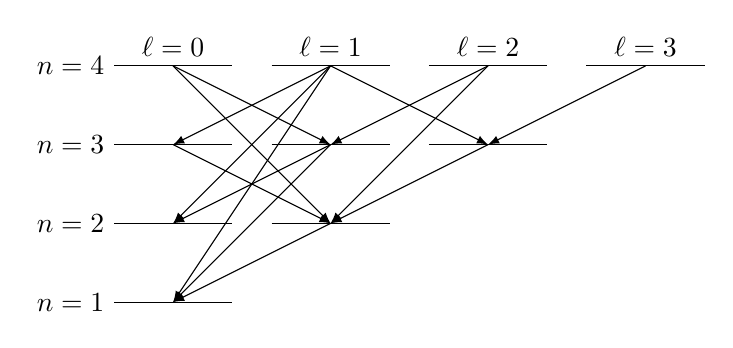
\begin{tikzpicture}
\pgfmathsetmacro{\kx}{1.5}
\pgfmathsetmacro{\ky}{1}
\pgfmathsetmacro{\ks}{0.5}
\draw[] (0,0) node[left]{$n=1$} --++ (\kx,0);
%
\draw[] (0,\ky) node[left]{$n=2$} --++ (\kx,0);
\draw[] (\kx+\ks,\ky) --++ (\kx,0);
%
\draw[] (0,2*\ky) node[left]{$n=3$} --++ (\kx,0);
\draw[] (\kx+\ks,2*\ky) --++ (\kx,0);
\draw[] (2*\kx+2*\ks,2*\ky) --++ (\kx,0);
%
\draw[] (0,3*\ky) node[left]{$n=4$} --++ (\kx,0) node[pos=0.5,above]{$\ell=0$};
\draw[] (\kx+\ks,3*\ky) --++ (\kx,0)node[pos=0.5,above]{$\ell=1$};
\draw[] (2*\kx+2*\ks,3*\ky) --++ (\kx,0)node[pos=0.5,above]{$\ell=2$};
\draw[] (3*\kx+3*\ks,3*\ky) --++ (\kx,0)node[pos=0.5,above]{$\ell=3$};
%
\draw[-latex] (\kx/2,3*\ky) --++ (\kx+\ks,-\ky);
\draw[-latex] (\kx/2,3*\ky) --++ (\kx+\ks,-2*\ky);
%
\draw[-latex] (\kx+\ks+\kx/2,3*\ky) --++ (-\kx-\ks,-\ky);
\draw[-latex] (\kx+\ks+\kx/2,3*\ky) --++ (-\kx-\ks,-2*\ky);
\draw[-latex] (\kx+\ks+\kx/2,3*\ky) --++ (-\kx-\ks,-3*\ky);
\draw[-latex] (\kx+\ks+\kx/2,3*\ky) --++ (\kx+\ks,-\ky);
%
\draw[-latex] (2*\kx+2*\ks+\kx/2,3*\ky) --++ (-\kx-\ks,-\ky);
\draw[-latex] (2*\kx+2*\ks+\kx/2,3*\ky) --++ (-\kx-\ks,-2*\ky);
%
\draw[-latex] (3*\kx+3*\ks+\kx/2,3*\ky) --++ (-\kx-\ks,-\ky);
%
\draw[-latex] (0*\kx+0*\ks+\kx/2,2*\ky) --++ (\kx+\ks,-\ky);
%
\draw[-latex] (1*\kx+1*\ks+\kx/2,2*\ky) --++ (-\kx-\ks,-\ky);
\draw[-latex] (1*\kx+1*\ks+\kx/2,2*\ky) --++ (-\kx-\ks,-2*\ky);
%
\draw[-latex] (2*\kx+2*\ks+\kx/2,2*\ky) --++ (-\kx-\ks,-1*\ky);
%
\draw[-latex] (1*\kx+1*\ks+\kx/2,1*\ky) --++ (-\kx-\ks,-1*\ky);
\end{tikzpicture}
\caption{ہائیڈروجن کی اولین چار سطحوں کا اجازتی تنزل۔}
\label{شکل_تابع_وقت_اضطراب_اجازتی_تنزل}
\end{figure} 

 
 
\ابتدا{سوال}\شناخت{سوال_تابع_مضطرب_اخذ_کریں}
مساوات \حوالہ{مساوات_تابع_مضطرب_ماخوذ_ث} میں دی گئی مقلوبی رشتہ ثابت کریں۔ \ترچھا{ اشارہ:} پہلے درج ذیل دکھائیں۔
\begin{align*}
	[L^2, z] = 2i\hslash(xL_y-yL_x-i\hslash z)
\end{align*}
اس کے ساتھ \عددی{\kvec{r}\cdot\kvec{L} =\kvec{r}\cdot(\kvec{r}\times\kvec{p}) = 0} استعمال کر کے درج ذیل دکھائیں۔
\begin{align*}
[L^2, [L^2, z]] = 2\hslash^2(zL^2+L^2z)	
\end{align*}
\عددی{z} سے \عددی{\kvec{r}} تک عمومیت دینا ایک آسان کام ہے۔
\انتہا{سوال}
\ابتدا{سوال}\شناخت{سوال_تابع_مضطرب_پیچیدگی_ختم}
دکھائیں کہ \عددی{\ell '= \ell = 0} کی صورت میں \عددی{\langle n'\ell'm'|\kvec{r}|n\ell m \rangle = 0} ہوگا۔ یوں مساوات \حوالہ{مساوات_تابع_مضطرب_ماخوذ_خ} میں درپیش \قول{کمزوری} ختم ہوتی ہے۔
\انتہا{سوال}
\ابتدا{سوال}
ہائیڈروجن کے \عددی{n = 3}، \عددی{\ell = 0}، \عددی{m = 0} حال میں ایک الیکٹران زمینی حال تک ( برقی جفت قطبی) تحویلی تسلسل کے ذریعہ پہنچتا ہے۔
\begin{enumerate}[a.]
\item
 اس تنزل کے لیے کونسی راہیں کھلی ہیں؟ انہیں درج ذیل صورت میں پیش کریں۔
\begin{align*}
	|300\rangle\to | n\ell m\rangle\to | n'\ell'm'\rangle\to\dots\to|100\rangle
\end{align*}
\item
 اگر آپ کے پاس، اس حال میں جوہروں سے بھرا ہوا ایک بوتل ہو، تب ہر راہ سے کتنا حصہ گزرے گا؟
\item
 اس حال کا عرصہ حیات کیا ہوگا؟ \ترچھا{اشارہ:} پہلی تحویل کے بعد یہ حال \عددی{|300\rangle} میں نہیں ہوگا، لہٰذا ہر تسلسل کا صرف پہلا قدم، عرصہ حیات کے حصول میں کام آئے گا۔ متعدد تحویلی راستوں کی صورت میں تمام تحویلی شرحوں کا مجموعہ لینا ہو گا۔
 \end{enumerate}
\انتہا{سوال}

%======================
\جزوحصہء{اضافی سوالات برائے باب \حوالہ{باب_تابع_وقت_نظریہ_اضطراب}}
\ابتدا{سوال}\شناخت{سوال_تابع_مضطرب_دیگر_قطع_نظر}
متعدد سطحی نظام کے لیے مساوات \حوالہ{مساوات_تابع_مضطرب_دو_سطحی} اور مساوات \حوالہ{مساوات_تابع_مضطرب_عمودیت}
\begin{align}
	H_0\psi_n = E_n\psi_n,\quad \langle \psi_n|\psi_m \rangle = \delta_{nm}
\end{align}
کو عمومیت دیتے ہوئے تابع وقت نظریہ اضطراب مرتب کریں۔ لمحہ \عددی{t=0} پر ہم اضطراب \عددی{H'(t)} چالو کرتے ہیں؛ یوں کل ہیملٹنی درج ذیل ہوگی۔
\begin{align}
	H = H_0 + H'(t)
\end{align}
\begin{enumerate}[a.]
\item
 مساوات \حوالہ{مساوات_تابع_مضطرب_وقت} کو درج ذیل تعمیمی روپ دیں
\begin{align}
	\Psi(t) = \sum c_n(t)\psi_ne^{-iE_nt/\hslash}
\end{align}
اور دکھائیں کہ
\begin{align}\label{مساوات_تابع_مضطرب_تفرق_شرح_مستقل}
	\dot{c}_m = -\frac{i}{\hslash}\sum_{n} c_nH'_{mn}e^{i(E_m-E_n)t/\hslash}
\end{align}
ہو گا، جہاں \عددی{H'_{mn}} درج ذیل ہے۔
\begin{align}
	H'_{mn} \equiv \langle \psi_m\abs{H'}\psi_n \rangle
\end{align}
\item
اگر نظام حال \عددی{\psi_N} سے آغاز کرے، تو دکھائیں کہ (اول رتبی نظریہ اضطراب میں) 
\begin{align}
	c_N(t)\cong1-\frac{i}{\hslash}\int_{0}^{t}H'_{NN}(t')\dif t'
\end{align}
اور درج ذیل ہوگا۔
\begin{align}
	c_m(t)&\cong-\frac{i}{\hslash}\int_{0}^{t}H'_{mN}(t')e^{i(E_m-E_N)t'/\hslash}\dif t'&& (m\neq N)
\end{align}
\item
 فرض کریں، ( لمحہ \عددی{t=0} پر چالو اور بعد میں لمحہ \عددی{t} پر منقطع کرنے کے علاوہ) \عددی{H'} \ترچھا{ مستقل} ہے۔ حال \عددی{N} سے حال \عددی{M} جہاں \عددی{M\neq N} ہے، میں تحویل کے احتمال کو \عددی{t} کا تفاعل لکھیں۔\ترچھا{ جواب:}
\begin{align}
	4\abs{H'_{MN}}^2\frac{\sin^2[(E_N-E_M)t/2\hslash]}{(E_N-E_M)^2}
\end{align}
\item
 فرض کریں \عددی{H'} وقت کا سائن نما تفاعل: \عددی{H'=V\cos(\omega t)} ہے۔ عمومی مفروضے فرض کرتے ہوئے دکھائیں کہ صرف توانائی \عددی{E_M = E_N\pm\hslash\omega} کے حالات میں تحویل ہو سکتی ہے اور ان کا احتمال درج ذیل ہے۔
\begin{align}
	P_{N\to M} = \abs{V_{MN}}^2\frac{\sin^2[(E_N-E_M\pm\hslash\omega)t/2\hslash]}{(E_N-E_M\pm\hslash\omega)^2}
\end{align}
\item
 فرض کریں کہ متعدد سطحی نظام پر غیر اتساقی برقناطیسی روشنی ڈالی جاتی ہے۔ حصہ \حوالہ{حصہ_تابع_مضطرب_غیر_اتساقی_اضطراب} کو دیکھتے ہوئے دکھائیں کہ تحرک شدہ اخراج کی تحویلی شرح وہی دو سطحی نظام کا کلیہ (مساوات \حوالہ{مساوات_تابع_مضطرب_شرح_بی_تا_اے}) دیگا۔
 \end{enumerate}
\انتہا{سوال}
\ابتدا{سوال}
عددی سر \عددی{c_m(t)} کو رتبہ اول تک سوال \حوالہ{سوال_تابع_مضطرب_دیگر_قطع_نظر} کے جزو -ج اور جزو- د کے لیے تلاش کریں۔ معمول زنی شرط:
\begin{align}
	\sum_{m}\abs{c_m(t)}^2 = 1
\end{align}
کی تصدیق کر کے، تضاد اگر موجود ہو، پر تبصرہ کریں۔ فرض کریں آپ ابتدائی حال \عددی{\psi_N} میں رہنے کا احتمال جاننا چاہتے ہیں؛ کیا \عددی{\abs{c_N(t)}^2} یا \عددی{1-\sum_{m\neq N}\abs{c_m(t)}^2} کا استعمال بہتر ثابت ہوگا؟
\انتہا{سوال}
%KKK edited till here 12 feb 2022
\ابتدا{سوال}
لامتناہی چوکور کنویں کے \عددی{N}ویں حال میں (وقت \عددی{t=0} پر ) ایک ذرہ آغاز کرتا ہے۔ وقتی طور پر کنویں کی تہہ بلند ہو کر واپس اپنی جگہ نیچے بیٹھتی ہے، جس کے تحت کنویں کے اندر مخفیہ یکساں ضرور لیکن تابع وقت ہوگا: \عددی{V_0(t)}، جہاں \عددی{V_0(0) = V_0(T) = 0} ہوگا۔
\begin{enumerate}[a.]
\item
مساوات \حوالہ{مساوات_تابع_مضطرب_تفرق_شرح_مستقل} استعمال کر کے \عددی{c_m(t)} کی ٹھیک ٹھیک قیمت دریافت کریں، اور دکھائیں کہ تفاعل موج کی \ترچھا{ ہیّت} تبدیل ہوگی لیکن کوئی تحویل نہیں ہوگی۔ تفاعل \عددی{V_0(t)} کی صورت میں تبدیلی ہیّت، \عددی{\psi(T)}، تلاش کریں۔
\item
 اسی مسئلے کو رتبہ اول نظریہ اضطراب سے حل کر کے دونوں نتائج کا موازنہ کریں۔

\ترچھا{تبصرہ:} جب بھی مخفیے کے ساتھ اضطراب ایک مستقل ( \عددی{x} میں مستقل نہ کے \عددی{t} میں) جمع کرتا ہو، یہی نتیجہ حاصل ہوگا؛ یہ صرف لامتناہی چوکور کنویں کی خاصیت نہیں ہے۔ سوال \حوالہ{سوال_تفاعل_موج_مستقل_جمع} کے ساتھ موازنہ کریں۔
\end{enumerate}
\انتہا{سوال}
\ابتدا{سوال}
ابتدا میں (یک بُعدی لامتناہی) چوکور کنویں کے زمینی حال میں کمیت \عددی{m} کا ایک ذرہ پایا جاتا ہے۔ لمحہ \عددی{t=0} پر ایک \قول{اینٹ} اس کنویں میں گرائی جاتی ہے، جس سے مخفیہ درج ذیل ہو جاتا ہے، جہاں \عددی{V_0\ll E_1} ہے۔
\begin{align*}
	V(x)=
	\begin{cases}
		V_0 & 0\leq x\leq a/2 \\
		0 & a/2<x\leq a \\
		\infty & \text{\RL{بصورت دیگر}}
	\end{cases}
\end{align*}
کچھ وقت \عددی{T} کے بعد، اینٹ ہٹائی جاتی ہے، اور ذرے کی توانائی ناپی جاتی ہے۔ (رتبہ اول نظریہ اضطراب میں) نتیجہ \عددی{E_2} ہونے کا احتمال کیا ہوگا؟
\انتہا{سوال}
\ابتدا{سوال}
ہم تحرک شدہ اخراج، (تحرک شدہ) انجذاب، اور ازخود اخراج دیکھ چکے ہیں۔ ازخود \ترچھا{ انجذاب} کیوں نہیں پایا جاتا ہے؟
\انتہا{سوال}
\ابتدا{سوال}\شناخت{سوال_تابع_مضطرب_گمک}
\اصطلاح{مقناطیسی گمک}۔\فرہنگ{مقناطیسی گمک}\حاشیہب{magnetic resonance}\فرہنگ{magnetic resonance} ساکن مقناطیسی میدان \عددی{B_0\ak} میں، \عددی{1/2} چکر کا ایک ذرہ جس کی مسکن مقناطیسی نسبت \عددی{\gamma} ہو، لارمر تعدد \عددی{\omega_0 = \gamma B_0} (مثال \حوالہ{مثال_تین_ابعادی_لارمر_استقبالی_حرکت}) سے استقبالی حرکت کرتا ہے۔ اب ہم ایک کمزور عرضی ریڈیائی تعدد میدان، \عددی{B_{r}[\cos(\omega t)\ai-\sin(\omega t)\aj]}، چالو کرتے ہیں جس سے کل میدان درج ذیل ہو جاتا ہے۔
\begin{align}
	\kvec{B} = B_{r}\cos(\omega t)\ai - B_{r}\sin(\omega t)\aj + B_0\ak
\end{align} 
\begin{enumerate}[a.]
\item
اس نظام کے لیے \عددی{2\times2} ہیملٹنی قالب (مساوات \حوالہ{مساوات_تین_ابعادی_جفت_قطب_ہیملٹنی}) تیار کریں۔
\item
 وقت \عددی{t} پر چکری حال \عددی{\chi(t) =\big( \begin{smallmatrix}a(t) \\b(t)\end{smallmatrix}\big)} ہونے کی صورت میں درج ذیل دکھائیں
\begin{align}
	\dot{a} = \frac{i}{2}\big(\Omega e^{i\omega t}b+\omega_0 a\big); \quad\dot{b} = \frac{i}{2}\big(\Omega e^{-i\omega t}a-\omega_0 b\big)
\end{align}
جہاں \عددی{\Omega\equiv\gamma B_{r}} کا تعلق ریڈیائی تعدد میدان کے زور سے ہے۔
\item
 ابتدائی قیمتوں \عددی{a_0} اور \عددی{b_0} کی صورت میں \عددی{a(t)} اور \عددی{b(t)} کا عمومی حل تلاش کریں۔ \ترچھا{جواب:} 
\begin{align*}
	a(t) &= \bigg\{a_0\cos(\omega't/2)+\frac{i}{\omega'}[a_0(\omega_0-\omega)+b_0\Omega]\sin(\omega't/2)\bigg\}e^{i\omega t/2} \\
	b(t) &= \bigg\{b_0\cos(\omega't/2)+\frac{i}{\omega'}[b_0(\omega-\omega_0)+a_0\Omega]\sin(\omega't/2)\bigg\}e^{-i\omega t/2} 
\end{align*}
جہاں درج ذیل ہوگا۔
\begin{align}
	\omega'\equiv\sqrt{(\omega-\omega_0)^2+\Omega^2}
\end{align}
\item
 ایک ذرہ ہم میدان چکری حال ( \عددی{a_0 = 1}، \عددی{b_0 = 0}) سے آغاز کرتا ہے۔ مخالف میدان چکر میں تحویل کے احتمال کو بطور وقت کا تفاعل تلاش کریں۔

\ترچھا{جواب:} \عددی{P(t) = \{\Omega^2/[(\omega-\omega_0)^2+\Omega^2]\}\sin^2(\omega't/2)}
\item
\اصطلاح{منحنی گمک،}\فرہنگ{منحنی گمک}\حاشیہب{resonance curve}\فرہنگ{resonance curve}
\begin{align}
	P(\omega) = \frac{\Omega^2}{(\omega-\omega_0)^2+\Omega^2}
\end{align}
کو ( مقررہ \عددی{\omega_0} اور \عددی{\Omega} کے لئے) جبری تعدد \عددی{\omega} کے تفاعل کے طور پر ترسیم کریں۔ آپ دیکھیں گے کہ \عددی{\omega = \omega_0} پر اس کی اعظم قیمت پائی جاتی ہے۔\قول{ اعظم قیمت کی نصف پر پوری چوڑائی} \عددی{\Delta\omega} تلاش کریں۔
\item
 چونکہ \عددی{\omega_0 = \gamma B_0} ہے، لہٰذا ہم گمک کا تجرباتی مشاہدہ کر کے ذرے کے مقناطیسی جفت قطبی معیار اثر کا تعین کر سکتے ہیں۔ \اصطلاح{مرکزوی مقناطیسی گمک}\فرہنگ{مرکزوی مقناطیسی گمک}\حاشیہب{nmr, nuclear magnetic resonance}\فرہنگ{nuclear magnetic resonance}\فرہنگ{nmr} تجربہ میں نوریے کا \عددی{g} جزو ضربی، ایک ٹسلا \عددی{(\SI{1}{\tesla})}کے ساکن میدان اور ایک مائیکرو ٹسلا \عددی{(\SI{1}{\micro\tesla})} حیطے کے ریڈیائی تعدد میدان کی مدد سے، ناپا جاتا ہے۔ تعدد گمک کیا ہوگا؟ ( پروٹان کے مقناطیسی معیار اثر کے لیے حصہ \حوالہ{حصہ_غیر_تابع_مضطرب_نہایت_مہین_بٹوارا} دیکھیں۔) منحنی گمک کی چوڑائی تلاش کریں۔ ( اپنا جواب \عددی{\si{\hertz}} میں دیں۔)
 \end{enumerate}
\انتہا{سوال}
\ابتدا{سوال}\شناخت{سوال_تابع_مضطرب_فاصلاتی_تغیر}
میں نے مساوات \حوالہ{مساوات_تابع_مضطرب_بہت_چھوٹا_جوہر} میں جوہر کو ( روشنی کے طول موج سے) اتنا چھوٹا تصور کیا کہ میدان کے فضائی تغیر کو نظر انداز کیا جا سکتا تھا۔ حقیقی برقی میدان درج ذیل ہوگا۔
\begin{align}
\kvec{E}(\kvec{r},t) = E_0\cos(\kvec{k}\cdot \kvec{r}-\omega t)
\end{align}
اگر جوہر کا مرکز مبدا پر ہو، تب متعلقہ حجم پر \عددی{\kvec{k}\cdot\kvec{r}\ll 1} 
(\عددی{\abs{\kvec{k}}=2\pi/{\lambda}} لہٰذا \عددی{\kvec{k}\cdot\kvec{r}\sim r/{\lambda}\ll 1} ) ہوگا، جس کی بنا پر ہم اس جزو کو نظرانداز کر سکتے تھے۔ فرض کریں ہم اول رتبی درستگی:
\begin{align}
\kvec{E}(\kvec{r},t) = E_0[\cos(\omega t)+(\kvec{k}\cdot\kvec{r})\sin(\omega t)]
\end{align}
کو نظر انداز نہیں کرتے۔ اس کا پہلا جزو \اصطلاح{ اجازتی} (\اصطلاح{ برقی جفت قطبی}) \فرہنگ{تحویلات!اجازتی برقی جفت قطبی}\حاشیہب{allowed electric dipole transitions}\فرہنگ{transitions!allowed electric dipole} تحویلات دے گا جن پر متن میں بات کی چکی ہے؛ دوسرا جزو \اصطلاح{ ممنوعہ} ( \اصطلاح{مقناطیسی جفت قطبی}\فرہنگ{تحویلات!ممنوعہ مقناطیسی جفت قطبی}\فرہنگ{transitions!forbidden magnetic dipole}\حاشیہب{forbidden magnetic dipole transitions} اور \اصطلاح{برقی چو قطبی}\فرہنگ{ممنوعہ برقی جفت قطبی تحویلات}\حاشیہب{forbidden electric quadrupole transitions}\فرہنگ{transitions!forbidden electric quadrupole}) تحویلات دے گا ( \عددی{\kvec{k}\cdot\kvec{r}} کی مزید بڑی طاقتیں، مزید ممنوعہ تحویلات دیں گی، جو زیادہ بلند متعدد قطبی معیار اثر سے وابستہ ہوں گی)۔
\begin{enumerate}[a.]
\item
ممنوعہ تحویلات کی ازخود اخراجی شرح حاصل کریں ( تقطیب اور حرکت کے رخوں پر اوسط تلاش کرنے کی ضرورت نہیں، اگرچہ مکمل جواب کے لیے ایسا کرنا ضروری ہے)۔ \ترچھا{جواب:}
\begin{align}
	R_{b\to a} = \frac{q^2\omega^5}{\pi\epsilon_0\hslash c^5}|\langle a|(\kvecsub{a}{n}\cdot\kvec{r})(\ak\cdot \kvec{r})|b \rangle|^2
\end{align}
\item
 دکھائیں کہ یک بُعدی مرتعش کے لیے ممنوعہ تحویلات سطح \عددی{n} سے سطح \عددی{n-2} میں ہوں گی، اور تحویلی شرح (جس کا اوسط \عددی{\kvecsub{a}{n}} اور \عددی{\ak} پر حاصل کیا گیا ہو) درج ذیل ہوگی۔
\begin{align}
	R = \frac{\hslash q^2\omega^3n(n-1)}{15\pi\epsilon_0m^2c^5}
\end{align}
(\ترچھا{تبصرہ:} یہاں \عددی{\omega} سے مراد نوریہ کا تعدد ہے نہ کہ مرتعش کا تعدد۔) \قول{ اجازتی }شرح کے لحاظ سے \قول{ممنوعہ} شرح کی نسبت تلاش کریں اور اس اصطلاح پر تبصرہ کریں۔
\item
 دکھائیں کہ ہائیڈروجن میں ممنوعہ تحویل بھی \عددی{2S\to 1S} تحویل کی اجازت نہیں دیتی۔ ( یہ تمام بلند متعدد قطب کے لیے بھی درست ہوگا؛ غالب تنزل، در حقیقت، دو نوریہ اخراج کی بنا پر ہوگا، جس کا عرصہ حیات تقریباً ایک سیکنڈ کا دسواں حصہ ہوگا۔)
 \end{enumerate}
\انتہا{سوال}
\ابتدا{سوال}
دکھائیں کہ \عددی{n,\ell } سے \عددی{n', \ell '} میں تحویل کے لیے ہائیڈروجن کی ازخود اخراجی شرح (مساوات \حوالہ{مساوات_تابع_مضطرب_خود_با_خود_شرح_حتمی}) درج ذیل ہوگی
\begin{align}
	\frac{e^2\omega^3I^2}{3\pi\epsilon_0\hslash c^3}\times
	\begin{cases}
		\frac{\ell +1}{2\ell +1}, & \ell '= \ell +1 \\
		\frac{\ell }{2\ell -1}, & \ell '= \ell -1 
	\end{cases}
\end{align}
جہاں \عددی{I} درج ذیل ہے۔
\begin{align}
	I\equiv\int_{0}^{\infty} r^3R_{n\ell }(r)R_{n'\ell '}(r)\dif r
\end{align}
(جوہر \عددی{m} کی کسی مخصوص قیمت سے آغاز کر کے کسی ایک \عددی{m'} حال میں، انتخابی قواعد:
\begin{align*}
m'=m-1,\quad m'=m,\quad m'=m+1
\end{align*}
 کے تحت، پہنچتا ہے۔ دھیان رہے کہ جواب \عددی{m} کا تابع نہیں۔) \ترچھا{ اشارہ:} پہلے \عددی{\ell '= \ell +1} صورت کے لیے \عددی{| n\ell m\rangle} اور \عددی{| n'\ell'm'\rangle} کے بیچ \عددی{x}، \عددی{y}، اور \عددی{z} کے تمام غیر صفر قالبی ارکان معلوم کریں۔ ان سے درج ذیل مقدار کا تعین کریں۔
\begin{align*}
	|\langle n', \ell +1,m+1|\kvec{r}|n\ell m \rangle|^2 + |\langle n', \ell +1, m|\kvec{r}|n\ell m \rangle|^2+|\langle n', \ell +1, m-1|\kvec{r}|n\ell m\rangle|^2
\end{align*}
یہی کچھ \عددی{\ell '= \ell -1} کے لیے بھی کریں۔
\انتہا{سوال}

%===================
